%% LyX 2.2.4 created this file.  For more info, see http://www.lyx.org/.
%% Do not edit unless you really know what you are doing.
\documentclass[12pt,english,british,reqno]{amsart}
\usepackage[T1]{fontenc}
\usepackage[latin9]{inputenc}
\pagestyle{plain}
\setcounter{secnumdepth}{4}
\setcounter{tocdepth}{1}
\usepackage{color}
\usepackage{babel}
\usepackage{float}
\usepackage{textcomp}
\usepackage{mathtools}
\usepackage{bm}
\usepackage{amstext}
\usepackage{amsthm}
\usepackage{amssymb}
\usepackage{graphicx}
\usepackage{setspace}
\usepackage[numbers]{natbib}
\onehalfspacing
\usepackage[unicode=true,
 bookmarks=true,bookmarksnumbered=false,bookmarksopen=true,bookmarksopenlevel=1,
 breaklinks=true,pdfborder={0 0 1},backref=false,colorlinks=false]
 {hyperref}
\hypersetup{pdftitle={Cloud Migration},
 pdfauthor={Andrea Decorte},
 pdfsubject={Cloud Computing},
 pdfkeywords={cloud, SCE, migration, enterprise, IBM}}
\usepackage{breakurl}

\makeatletter

%%%%%%%%%%%%%%%%%%%%%%%%%%%%%% LyX specific LaTeX commands.
%% Because html converters don't know tabularnewline
\providecommand{\tabularnewline}{\\}

%%%%%%%%%%%%%%%%%%%%%%%%%%%%%% Textclass specific LaTeX commands.
\numberwithin{equation}{section}
\numberwithin{figure}{section}
\theoremstyle{plain}
\newtheorem{thm}{\protect\theoremname}
  \theoremstyle{definition}
  \newtheorem{defn}[thm]{\protect\definitionname}
  \theoremstyle{remark}
  \newtheorem{rem}[thm]{\protect\remarkname}

%%%%%%%%%%%%%%%%%%%%%%%%%%%%%% User specified LaTeX commands.
\DeclareRobustCommand{\gobblefour}[5]{}
\newcommand*{\SkipTocEntry}{\addtocontents{toc}{\gobblefour}}
\usepackage{natbib}
\usepackage{color}
\usepackage[geometry]{ifsym}
\AtBeginDocument{\let\origref\ref
   \renewcommand{\ref}[1]{(\origref{#1})}}
\definecolor{Code}{rgb}{0.1,0.1,0.1}
\definecolor{Decorators}{rgb}{0.7,0,0.7}
\definecolor{Numbers}{rgb}{0.5,0,0}
\definecolor{MatchingBrackets}{rgb}{0.25,0.5,0.5}
\definecolor{Keywords}{rgb}{0,0,1}
\definecolor{self}{rgb}{.87,.46,0}
\definecolor{Strings}{rgb}{0,0.66,0}
\definecolor{Comments}{rgb}{0.388,0.4705,0.518}
\definecolor{Backquotes}{rgb}{0,0,0}
\definecolor{Classname}{rgb}{0,0,0}
\definecolor{FunctionName}{rgb}{0,0,0}
\definecolor{Operators}{rgb}{0,0,0}
\definecolor{Background}{rgb}{0.99,0.99,0.99}
% Added by lyx2lyx
\renewcommand{\textendash}{--}
\renewcommand{\textemdash}{---}

\@ifundefined{showcaptionsetup}{}{%
 \PassOptionsToPackage{caption=false}{subfig}}
\usepackage{subfig}
\makeatother

\usepackage{listings}
\lstset{language=Python,
frame=trBL,
xleftmargin=3ex,
xrightmargin=3ex,
linewidth=15cm,
framextopmargin=1em,
framexbottommargin=1em,
showspaces=false,
showtabs=false,
showstringspaces=false,
tabsize=4,
basicstyle={\ttfamily\tiny},
backgroundcolor={\color{Background}},
commentstyle={\color{Comments}\slshape},
stringstyle={\color{Strings}},
morecomment={[s][\color{Strings}]{"""}{"""}},
morecomment={[s][\color{Strings}]{'''}{'''}},
keywordstyle={\color{Keywords}\bfseries},
keywordstyle={[2]\color{Decorators}},
emph={self},
emphstyle={\color{self}\slshape},
moredelim={**[s][\bfseries]{class }{:}},
moredelim={**[s][\bfseries]{def }{:}},
moredelim={**[s][\mdseries]{(}{)}}}
  \addto\captionsbritish{\renewcommand{\definitionname}{Definition}}
  \addto\captionsbritish{\renewcommand{\remarkname}{Remark}}
  \addto\captionsbritish{\renewcommand{\theoremname}{Theorem}}
  \addto\captionsenglish{\renewcommand{\definitionname}{Definition}}
  \addto\captionsenglish{\renewcommand{\remarkname}{Remark}}
  \addto\captionsenglish{\renewcommand{\theoremname}{Theorem}}
  \providecommand{\definitionname}{Definition}
  \providecommand{\remarkname}{Remark}
\addto\captionsbritish{\renewcommand{\lstlistingname}{Listing}}
\addto\captionsenglish{\renewcommand{\lstlistingname}{Listing}}
\providecommand{\theoremname}{Theorem}
\renewcommand{\lstlistingname}{Listing}

\begin{document}

%%FRONT PAGE
%\begin{titlepage}
%upper part
\begin{center}
{{\Large{\textsc{Universit\`a degli studi di Torino \\}}}} \vspace{5mm} {\small{\bf SCUOLA DI SCIENZE DELLA NATURA\\ \vspace{3mm}
Corso di Laurea Magistrale in Fisica dei Sistemi Complessi}}
\vspace{5mm}
\end{center}
%logo
\begin{center}

\includegraphics[scale=.3]{head/logo.png}
\end{center}
%title
\begin{center}
\vspace{5mm}
{\large{\bf Tesi di Laurea Magistrale\\}}
\vspace{5mm}
{\LARGE{\bf Discrete and continuous models of spatial evolutionary games\\}}
%\vspace{5mm}
%{\LARGE{\bf SECOND ROW TITLE}}
\end{center}
\vspace{20mm}
%relatore
\par
\noindent
\begin{minipage}[t]{0.47\textwidth}
{\large{\bf Relatore:\\
Chiar.mo Prof.\\
Cermelli Paolo}}
\vspace{8mm}
%{\large{\bf \\ Controrelatore:\\
%Prof.\\
%Zio Paperone}}
\end{minipage}
\hfill
\begin{minipage}[t]{0.47\textwidth}\raggedleft
\vspace{20mm}
{\large{\bf Candidato:\\
Dell'Orto Alessandro}}
\end{minipage}
\vspace{10mm}
\begin{center}
{\large{\bf 
Anno Accademico 2019/2020}}
\end{center}

\end{titlepage}

\begin{titlepage}
%upper part
\begin{center}
{{\Large{\textsc{Universit\`a degli studi di Torino \\}}}} \vspace{5mm} {\small{\bf SCUOLA DI SCIENZE DELLA NATURA\\ \vspace{2mm}
 Dipartimento di Fisica\\ \vspace{2mm} Corso di Laurea Magistrale in Fisica dei Sistemi Complessi}}
\vspace{5mm}
\end{center}
%logo
\begin{center}

\includegraphics[scale=.3]{head/logo.png}
\end{center}
%title
\begin{center}
\vspace{5mm}
{\large{\bf Tesi di Laurea Magistrale\\}}
\vspace{5mm}
{\LARGE{\bf Discrete and continuous models of \\ spatial evolutionary games}}
%\vspace{5mm}
%{\LARGE{\bf SECOND ROW TITLE}}
\end{center}
\vspace{10mm}
%reatori e candidato
\vspace{10mm}
\par
\noindent
\begin{minipage}[t]{0.47\textwidth}
{\large{\bf Relatore:\\
Prof. Paolo Cermelli}}\\
\vspace{2mm}
{\large{\bf \\ Controrelatore:\\
Dott. Matteo Osella}}
\end{minipage}
\hfill
\begin{minipage}[t]{0.47\textwidth}\raggedleft
\vspace{8mm}
{\large{\bf Candidato:\\
Alessandro Dell'Orto}}
\end{minipage}
\vspace{8mm}
\begin{center}
{\large{\bf 
Anno Accademico 2019/2020}}
\end{center}

\end{titlepage}


%%DEDICATION (the initial quote)
\thispagestyle{empty}
\begin{flushright}

\vspace*{60mm}

To whom I love





\end{flushright}


\pagebreak{}

\thispagestyle{empty}

\selectlanguage{english}%
\SkipTocEntry

\section*{Abstract}

Since 1950, the Prisoner's Dilemma was used as an ideal model to study
the cooperative behaviour in social and biological systems. The aim
of this work is to study and compare discrete-agents and continuous
models for the spatial evolutionary game. First, we analyze and solve
numerically the known PDE models for the spatial Prisoner's Dilemma:
the reaction-diffusion equation of Vickers (1989) and then the hyperbolic
model proposed by Amadori, Boccabella e Natalini (2010). We discuss
the relations between the solutions of these PDEs and discrete models
of random walkers on a square lattice evolving according to the replicator
equation. We finally study the model of Durrett (2014), who showed
that spatial games on lattices can be written as a perturbed voter
model and that they converge to the solutions of a reaction-diffusion
replicator equation of a modified game. Following this approach, after
simulating a perturbed voter model on a simple lattice we propose
a reaction-diffusion equation in two spatial dimensions for a modified
game and solve it numerically.\selectlanguage{british}%



\pagebreak{}

\pagenumbering{roman}

\tableofcontents{}

\pagebreak{}

\pagenumbering{arabic}
\setcounter{page}{1}

\cleardoublepage

\part*{Introduction}
\noindent \begin{flushright}
\textit{A less obvious type of application (of non-cooperative}\\
\textit{ games) is to the study of cooperative games.}\\
John Forbes Nash Jr.
\par\end{flushright}

Since 1950, the prisoner's dilemma was used as the ideal model to
study the cooperative behaviours in a biological context. Its original
formulation can be expressed as follows \citep{wiki}:

\medskip{}

\noindent \textit{}%
\noindent\begin{minipage}[t]{1\columnwidth}%
\noindent \textit{Two members of a criminal gang are arrested and
imprisoned. Each prisoner is in solitary confinement with no means
of communicating with the other. The prosecutors lack sufficient evidence
to convict the pair on the principal charge, but they have enough
to convict both on a lesser charge. Simultaneously, the prosecutors
offer each prisoner a bargain. Each prisoner is given the opportunity
either to betray the other by testifying that the other committed
the crime, or to cooperate with the other by remaining silent. The
possible outcomes are: }
\begin{itemize}
\item \textit{If only one of them betrays and the other remains silent;
the former will be set free and the latter will serve 7 years in prison.}
\item \textit{If both betray the other, each of them serves 6 years in prison.}
\item \textit{If both remain silent, both of them will serve only 1 year
in prison.}
\end{itemize}
%
\end{minipage}

\medskip{}

In a formal way, we can define the prisoner's dilemma using the following
payoff matrix:

\[
A=\left[\begin{array}{cc}
\left(R,R\right) & \left(S,T\right)\\
\left(T,S\right) & \left(P,P\right)
\end{array}\right]
\]

Where in the above example, $R=-1$, $S=-7$, $T=0$ e $P=-6$. It
can be shown that the properties of the game do not change if we choose
$S=P=0$, $R=1$ e $T=b$, and being a symmetric game we can simplify:
\[
A=\left(\begin{array}{cc}
1 & 0\\
b & 0
\end{array}\right)
\]
with $b\geq1$. 

In 1973 the work of Maynard Smith and Price \citep{MaynardSmith1973}
started the evolutionary game theory and in 1978 Taylor and Jonker
\citep{TaylorJ78} wrote the replicator equation:
\[
\dot{p}_{\ell}=p_{\ell}\left[\mathbf{e}_{\ell}^{T}A\,\mathbf{p}-\mathbf{p}^{T}A\,\mathbf{p}\right]
\]
where $p_{\ell}$ is the frequency of strategy $\ell$; $\mathbf{e}_{\ell}^{T}A\,\mathbf{p}$
is the payoff of the focal player playing the strategy $\ell$ against
the population playing the mixed strategy $\mathbf{p}$; $\mathbf{p}^{T}A\,\mathbf{p}$
is the payoff of the focal player playing the same mixed strategy
$\mathbf{p}$ of the population. 

In the last three decades, the spatial version of the evolutionary
game has been extensively studied and now there are several models
(not always coherent with each other). 

In this work, we will study four of these models and proceed as follows:
\begin{enumerate}
\item In the first chapter we will study and solve numerically two continuous
models:
\begin{enumerate}
\item In 1989, Vickers \citep{vickers_spatial_1989} wrote a reaction-diffusion
equation describing a spatial dynamics of the game:
\[
\frac{\partial n_{\ell}}{\partial t}=n_{\ell}\left[\frac{\mathbf{e}_{\ell}^{T}A\,\mathbf{n}}{N}-\frac{\mathbf{n}^{T}A\,\mathbf{n}}{N^{2}}\right]+D_{\ell}\nabla^{2}n_{\ell}\qquad\ell=1,2
\]
 where $N\left(\mathbf{x},t\right)=\sum_{\ell=1}^{n}n_{\ell}$ is
the total density, $D_{\ell}$ is the diffusion coefficient for $\ell-th$
strategy and $n_{\ell}$ is the number density per unit area of agents
using strategy $\ell$.
\item In 2010, Amadori, Boccabella and Natalini \citep{amadori_one_2010,amadori_hyperbolic_2011}
proposed a different equation, that corrected the infinite speed admitted
by the above equation:
\[
\begin{cases}
\frac{\partial n_{\ell}}{\partial t} & =-\bm{\nabla}\cdot\bm{\omega}_{\ell}+n_{\ell}\left[\frac{\mathbf{e_{\ell}}^{T}A\,\mathbf{n}}{N}-\frac{\mathbf{n}^{T}A\,\mathbf{n}}{N^{2}}\right]\\
\tau\frac{\partial\bm{\omega}_{\ell}}{\partial t} & =-\lambda_{\ell}^{2}\bm{\nabla}n_{\ell}-\bm{\omega}_{\ell}
\end{cases}\qquad\ell=1,2
\]
where $\bm{\omega}_{\ell}$ is the flux vector of the population $\ell$,
$\tau$ is the relaxation time and $\lambda_{\ell}^{2}$ is correlated
to diffusion coefficient.
\end{enumerate}
\item In the second chapter we will propose a discrete spatial version of
the replicator equation \citep{hofbauer_game_nodate}.
\item In the third chapter we shall study the model of Durrett \citep{durrett_spatial_2014,cox_voter_2011},
who showed that spatial games on lattices can be written as a perturbed
voter model and that they converge to the solutions of a reaction-diffusion
replicator equation of a modified game.
\end{enumerate}
In the first three models we simply observe that there is no survival
of cooperators and that the number of individuals decreases until
the extinction, but in the discrete one the speed of extinction is
the slowest. The simulation of the fourth model in $2D$ gives us
a complete consensus, or rather we observe no coexistence of cooperators
and defectors.


\part{The equations and the algorithms}
\noindent \begin{flushright}
\textit{Paradoxically, it has turned out that game theory}\\
\textit{ is more readily applied to biology than }\\
\textit{to the field of economic behaviour for which }\\
\textit{it was originally designed.}\\
\textit{ }John Maynard Smith 
\par\end{flushright}

As anticipated, after an introduction to the classical game theory
and the evolutionary game theory, this chapter aims to study two partial
differential equations (PDEs) and to solve them numerically. Numerical
methods for PDE is a chaotic world. To move in it, we have first to
determine what type of PDE we want to solve, and then work on the
order of accuracy desired. Thus, considering a generic PDE of the
form:
\[
A\frac{\partial^{2}u}{\partial x^{2}}+B\frac{\partial^{2}u}{\partial x\partial y}+C\frac{\partial^{2}u}{\partial y^{2}}+D\frac{\partial u}{\partial x}+E\frac{\partial u}{\partial y}+F=0
\]

\begin{itemize}
\item If $B^{2}-AC<0$, the PDE is elliptic;
\item If $B^{2}-AC=0$, the PDE is parabolic;
\item If $B^{2}-AC>0$, the PDE is hyperbolic.
\end{itemize}
Below, after an analysis of the equations, we define, verify and validate
numerical methods for the investigated PDEs, and finally solve them
numerically.

\section{Classical game theory}

Game theory is the study of mathematical models of conflict and cooperation
between intelligent rational decision-makers. It provides general
mathematical techniques for analyzing situations in which two or more
individuals make decisions that will influence one another's welfare
\cite{myerson1991game}.
\begin{defn}
A strategic form game is any triplet $\Gamma$ of the form:
\[
\Gamma=\left\{ N,\left(C_{\ell}\right)_{\ell\in\mathcal{N}},\left(u_{\ell}\right)_{\ell\in\mathcal{N}}\right\} ,
\]
 where:
\end{defn}

\begin{enumerate}
\item $\mathcal{N}$ is the nonempty set of \textit{simultaneous-playing
rational players} in the game;
\item $C_{\ell}$ is the nonempty set of strategies (or \textit{pure strategies})
available to player $\ell$. In a strategic-form game $\Gamma$ each
player $\ell$ must choose one of the strategies $c_{\ell}$ in the
set $C_{\ell}$. We let $C$ denote the set of all possible strategy
profiles, i.e. \[C=\underset{\ell\in\mathcal{N}}{\textifsym{\BigCross}} C_{\ell}\]
so a pure strategy profile is:
\[
\mathbf{c}\coloneqq\left(c_{\ell}:\ell\in\mathcal{N}\right)
\]
\item $u_{\ell}$ is the payoff function from $C$ into the set of real
numbers $\mathbb{R}$, i.e.:
\begin{align*}
u_{\ell}: & C\rightarrow\mathbb{R}\\
 & \mathbf{c}\mapsto u_{\ell}\left(\mathbf{c}\right)
\end{align*}
It represents the expected payoff that player $\ell$ would get in
this game if $\mathbf{c}$ were the combination of strategies implemented
by the players. 
\end{enumerate}
The games that involve only two players can be represented with a
more convenient form: the \textit{payoff matrix}. The player labeled
with $1$ is called \textit{row player} and the player labeled with
$2$ is called \textit{column player}. The rows of the payoff matrix
are the pure strategies of the row player, $C_{1}=\left(R_{1},\dots,R_{m}\right)$,
while the columns are the pure strategies of the column player, $C_{2}=\left(T_{1},\dots,T_{n}\right)$.
The element on the $i^{th}$ row and on the $j^{th}$column has a
pair of values that represents the pair of the payoffs related to
the strategy profile $\left(R_{i},T_{j}\right)$. For example, in
the prisoner's dilemma both the prisoners have $C_{1}=C_{2}=\left\{ cooperate,\quad defect\right\} $
\begin{center}
\begin{tabular}{|c|c|c|}
\hline 
 & cooperate & defect\tabularnewline
\hline 
\hline 
cooperate & R,R & S,T\tabularnewline
\hline 
defect & T,S & P,P\tabularnewline
\hline 
\end{tabular}
\par\end{center}

The concept of pure strategy can be extended, assuming that the players
can play their pure strategies with certain probabilities.
\begin{defn}
Let $\Delta\left(C_{\ell}\right)$ be the set of the probability measure,
i.e.:
\[
\Delta\left(C_{\ell}\right)=\left\{ \bm{\sigma}_{\ell}=\left(p_{1},\dots,p_{k}\right)\in\mathbb{R}^{k}:p_{\ell}\geq0,\ \sum_{\ell=1}^{k}p_{\ell}=1\right\} 
\]
A mixed strategy for player $\ell$ is any $\bm{\sigma}_{\ell}\in\Delta\left(C_{\ell}\right)$
that specifies a probability $\bm{\sigma}_{\ell}\left(c_{\ell}\right)$
for every $c_{\ell}$ that player $\ell$ could play. In other terms
$\bm{\sigma}_{\ell}$ is a $\left(k-1\right)-simplex$. So a mixed
strategy profile is:

\[\bm{\sigma}\coloneqq\left(\bm{\sigma}_{\ell}:\ell\in\mathcal{N}\right)\in\underset{\ell\in\mathcal{N}}{\textifsym{\BigCross}} \Delta \left(C_{\ell}\right) \]For
2-players games we denote the mixed strategies by:
\begin{align*}
\mathbf{p} & \in\Delta\left(C_{1}\right)\\
\mathbf{q} & \in\Delta\left(C_{2}\right).
\end{align*}
The payoff function of the player $i$ in terms of the mixed strategies
become\begin{align}u_{\ell}:&\underset{\ell\in\mathcal{N}}{\textifsym{\BigCross}}\Delta\left(C_{\ell}\right)\rightarrow\mathbb{R}\\&\bm{\sigma}\mapsto u_{\ell}\left(\bm{\sigma}\right)\end{align}
and it can be computed by:
\[
u_{\ell}\left(\bm{\sigma}\right)=\sum_{c\in C}\prod_{j\in\mathcal{N}}\bm{\sigma}_{j}\left(c_{j}\right)u_{\ell}\left(\mathbf{c}\right)
\]
\end{defn}

\begin{rem}
For games with 2 players, the payoff matrix allows us to compute the
payoff with a simple matrix multiplication, i.e.:
\[
u_{\ell}\left(\mathbf{p},\mathbf{q}\right)=\mathbf{p}{}^{T}A\mathbf{q}
\]
For example, consider the row player of the prisoner's dilemma playing
the strategy $\mathbf{p}=\left(\begin{array}{c}
p_{C}\\
p_{D}
\end{array}\right)$ against the column player playing $\mathbf{q}=\left(\begin{array}{c}
q_{C}\\
q_{D}
\end{array}\right)$ and its payoff matrix is:
\[
A=\left(\begin{array}{cc}
R & S\\
T & P
\end{array}\right)
\]
So, the payoff is:
\[
u_{1}\left({\bf p},{\bf q}\right)=\left(\begin{array}{cc}
p_{C} & p_{D}\end{array}\right)\left(\begin{array}{cc}
R & S\\
T & P
\end{array}\right)\left(\begin{array}{c}
q_{C}\\
q_{D}
\end{array}\right)
\]
 Note, we write the pure strategies as a vector ${\bf e_{\ell}}$
with $1$ on the $\ell-th$ component and zero otherwise. For instance,
the cooperate strategy in the prisoner's dilemma is:
\[
{\bf e}_{C}=\left(\begin{array}{c}
1\\
0
\end{array}\right).
\]
\end{rem}

Now, we can introduce one of the most important concept of the game
theory: the \textit{Nash equilibrium. }
\begin{defn}
Given a strategic form game:
\[
\Gamma=\left\{ N,\left(C_{\ell}\right)_{\ell\in\mathcal{N}},\left(u_{\ell}\right)_{\ell\in\mathcal{N}}\right\} ,
\]
 a mixed strategy profile:

\[\bm{\sigma}\coloneqq\left\{\bm{\sigma}_{\ell}:\ell\in\mathcal{N}\right\} \in \underset{\ell\in\mathcal{N}}{\textifsym{\BigCross}}\Delta\left(C_{\ell}\right)\]is
a Nash equilibrium if:
\[
\forall\ell\in\mathcal{N},\quad u_{\ell}\left(\bm{\sigma}_{-\ell}\,,\ \bm{\sigma}_{\ell}\right)\geq u_{\ell}\left(\bm{\sigma}_{-\ell}\,,\ \bm{\tau}\right)\qquad\forall\bm{\tau}\in\Delta\left(C_{\ell}\right)
\]
 where $\bm{\sigma}_{-\ell}$ denote the set of all strategies for
the players other than $\ell$. In 2 players games the mixed strategy
profile $\left(\mathbf{p}^{*},\,\mathbf{q}^{*}\right)\in\Delta\left(C_{1}\right)\times\Delta\left(C_{2}\right)$
is a Nash equilibrium if:
\begin{align*}
u_{1}\left(\mathbf{p}^{*},\,\mathbf{q}^{*}\right) & \geq u_{1}\left(\mathbf{p},\,\mathbf{q}^{*}\right)\qquad\forall\mathbf{p}\in\Delta\left(C_{1}\right)\\
u_{2}\left(\mathbf{p}^{*},\,\mathbf{q}^{*}\right) & \geq u_{2}\left(\mathbf{p}^{*},\,\mathbf{q}\right)\qquad\forall\mathbf{q}\in\Delta\left(C_{2}\right)
\end{align*}
\end{defn}

In other words, a Nash equilibrium is a situation in which none of
the players would want to change their strategy without the other
players changing theirs. 

We can now state the general existence theorem of Nash \cite{Nash1951}.
\begin{thm}
Given any game $\Gamma$ in strategic form with a finite number of
players and strategies, there exists at least one equilibrium in $\underset{\ell\in\mathcal{N}}{\textifsym{\BigCross}}\Delta\left(C_{\ell}\right)$.
\end{thm}


\section{Evolutionary game theory}

In 1973 the biologist John Maynard Smith and the mathematician G.
R. Price wrote an article in Nature showing how game theory applies
to the behaviour of animals \cite{MaynardSmith1973}. The keys of
their work are the following \cite{gintis_game_2009}:
\begin{itemize}
\item the strategy set of the players are the genotypic characteristics,
the phenotypic traits and the cultural inheritance of the individuals
of the species;
\item in place of the one-shot and repeated games of classical game theory,
we pick randomly an individual (called focal player) from a homogeneous
population and then observe what happens when the strategy of the
focal player varies;
\item the fitness of the focal player is seen as the payoff of the game;
\item the concept of the Nash equilibrium is not sufficient anymore, and
a new concept of equilibrium is introduced; namely we require that
a whole population using this ``new equilibrium'' strategy cannot
be invaded by a small \textit{mutant} group.
\end{itemize}
The revolution of the evolutionary games is the unneeded rationality
of the players, indeed it can be applied to every species and not
just the higher primates.

Now, we can formalize the whole problem. Consider a two-player strategic
form game in which both players have the same set of pure strategies
$C_{1}=C_{2}=C$ and are interchangeable, i.e. the payoffs to the
agent $1$ playing $c_{i}\in C$ and the player $2$ playing $c_{j}\in C$
are $u_{1}\left(c_{1},c_{2}\right)=u\left(c_{1},c_{2}\right)$ for
the first and $u_{2}\left(c_{1},c_{2}\right)=u\left(c_{2},c_{1}\right)$
for the second. We call this: a \textit{symmetric game}. In this case,
the payoff matrix represents only the payoffs for the row player,
because the payoffs to the column player are just the transpose. For
example, the prisoner's dilemma is clearly a symmetric game, and the
payoff matrix is simply:
\[
A=\left(\begin{array}{cc}
R & S\\
T & P
\end{array}\right)
\]
 In this context, the concept of mixed strategy as defined above is
quite meaningless. We can interpreter a mixed strategy $\mathbf{p}=\left(p_{1},\ldots,p_{k}\right)\in\Delta\left(C\right)$
as the \textit{state of the population}, i.e. $p_{\ell}$ is the proportion
of individuals of the population playing the pure strategy $c_{\ell}$. 

As anticipated, the notion of Nash equilibrium is not sufficient and
we need a more stringent condition.
\begin{defn}
A strategy $\mathbf{p}^{*}\in\Delta\left(C\right)$ is an \textit{evolutionary
stable strategy} (ESS) if the two following conditions are guaranteed:
\[
u\left(\mathbf{p}^{*},\,\mathbf{p}^{*}\right)\geq u\left(\mathbf{p},\,\mathbf{p}^{*}\right)\qquad\forall\mathbf{p}\in\Delta\left(C\right)
\]

\[
\exists\mathbf{p}'\,:\,u\left(\mathbf{p}^{*},\,\mathbf{p}^{*}\right)=u\left(\mathbf{p}',\,\mathbf{p}^{*}\right)\Rightarrow u\left(\mathbf{p}^{*},\,\mathbf{p}'\right)>u\left(\mathbf{p}',\,\mathbf{p}'\right)
\]
The first condition is the Nash equilibrium for symmetric games, while
the second one is said \textit{resistance to invasion}.
\end{defn}


\subsection{The replicator}

\textcolor{black}{To study an evolutionary system the best instrument
is the replicator, }\textit{\textcolor{black}{which is an entity having
some means of making approximately accurate copies of itself}}\textcolor{black}{{}
\cite{gintis_game_2009}. For example, a replicator can be a gene,
a belief, a phenotypic trait or more broadly a strategy in a game.}\textit{\textcolor{red}{{}
}}\textcolor{black}{In the evolutionary dynamic we study how the frequency
distribution of a set of replicators (in a particular environmental
setting and with a certain model of interaction) changes over time.}
There are several models to examine an evolutionary dynamic. We focus
our attention on the replicator dynamics proposed in 1978 by Taylor
and Jonker \cite{TaylorJ78}.

Assume that the population is divided into $n$ types with frequencies
$p_{1}$ to $p_{n}$ and that the fitness of the $\ell-th$ type is
a function of the state of the population $\mathbf{p}$. We may express
the rate of increase $\frac{\dot{p}_{\ell}}{p_{\ell}}$ of $\ell-th$
type as:
\[
\frac{\dot{p}_{\ell}}{p_{\ell}}=\ell^{th}type\ fitness-average\ fitness
\]
where the fitness of the $\ell-th$ type is $u\left(c_{\ell},\,\mathbf{p}\right)$
and the average one is $u\left(\mathbf{p},\,\mathbf{p}\right)$, so
we obtain the \textit{replicator equation:}
\begin{equation}
\dot{p}_{\ell}=p_{\ell}\left[u\left(c_{\ell},\,\mathbf{p}\right)-u\left(\mathbf{p},\,\mathbf{p}\right)\right]\qquad\ell=1,\ldots,\,n\ .\label{eq:replicator}
\end{equation}
of unknowns $p_{\ell}=p_{\ell}\left(t\right)$.
\begin{thm}
The replicator dynamics \ref{eq:replicator} has the following properties:
\begin{enumerate}
\item The simplex $\Delta$ is invariant under the replicator dynamics,
i.e. if $\mathbf{p}\left(0\right)\in\Delta$ then $\mathbf{p}\left(t\right)\in\Delta$
for all $t$ in the chosen interval.
\item If $\mathbf{p}^{*}$ is a Nash equilibrium of the symmetric game,
then $\mathbf{p}^{*}$ is a fixed point of the replicator dynamics. 
\item If $\mathbf{p}^{*}$is a stable equilibrium in the sense of Lyapunov
of the replicator dynamics, then it is a Nash equilibrium of the related
symmetric game.
\item The evolutionarily stable strategies are attractors of the replicator
dynamics.
\end{enumerate}
\end{thm}


\section{The parabolic dynamics\label{sec:Parabolic-dynamic}}

In 1989, Vickers \cite{vickers_spatial_1989} suggested a spatial
version of the replicator equation \ref{eq:replicator} by adding
a diffusive term, i.e. for the Prisoner's Dilemma:
\[
\frac{\partial p_{\ell}}{\partial t}=p_{\ell}\left[u\left(c_{\ell},\,\mathbf{p}\right)-u\left(\mathbf{p},\,\mathbf{p}\right)\right]+D_{\ell}\nabla^{2}p_{\ell}\qquad\ell=1,\,2
\]
where $p_{\ell}=p_{\ell}\left(\mathbf{x},t\right)$ the proportion
of individuals of the population playing the pure strategy $c_{\ell}$,
$\mathbf{x}$\footnote{We have a little abuse of notation. We use $x$ both to indicate the
vector $\mathbf{x}=\left(\begin{array}{c}
x\\
y
\end{array}\right)$ and the coordinate.} is the position vector and $D_{\ell}$ is the dispersal rate. Making
explicit the payoff, using the payoff matrix:
\begin{equation}
A=\left(\begin{array}{cc}
1 & 0\\
b & 0
\end{array}\right)\label{eq:payoff}
\end{equation}
we obtain:
\[
\frac{\partial p_{\ell}}{\partial t}=p_{\ell}\left[\mathbf{e}_{\ell}^{T}A\,\mathbf{p}-\mathbf{p}^{T}A\,\mathbf{p}\right]+D_{\ell}\nabla^{2}p_{\ell}\qquad\ell=1,\,2
\]
In this form, the evolution is not clear! Indeed, the equation is
defined on a simplex (two dimensional for the PD), thus if a solution
$p_{\alpha}\rightarrow1$, we have two possibilities:
\begin{enumerate}
\item the number of individuals of the population $\alpha$ is increasing
indefinitely and faster than any other (this hypothesis is not biologically
reasonable);
\item the number of the total population is constant, but $\alpha-type$
is increasing faster than any other type. 
\end{enumerate}
For this reason, Vickers proposed a modification of the model of the
form:
\begin{equation}
\frac{\partial n_{\ell}}{\partial t}=n_{\ell}\left[\frac{\mathbf{e}_{\ell}^{T}A\,\mathbf{n}}{N}-\frac{\mathbf{n}^{T}A\,\mathbf{n}}{N^{2}}\right]+D_{\ell}\nabla^{2}n_{\ell}\qquad\ell=1,\,2\label{eq:vick}
\end{equation}
where $n_{\ell}\left(\mathbf{x},t\right)$ is the number density per
unit area of the strategy $\ell$ in $\mathbf{x}$ at time $t$, and
\[
N=\sum_{i=1}^{n}n_{i}
\]
is the total number density. For the Prisoner's Dilemma we can write:
\begin{align*}
\frac{\partial N}{\partial t} & =\frac{\partial n_{1}}{\partial t}+\frac{\partial n_{2}}{\partial t}=n_{1}\left[\frac{\mathbf{e}_{1}^{T}A\,\mathbf{n}}{N}-\frac{\mathbf{n}^{T}A\,\mathbf{n}}{N^{2}}\right]\\
 & +n_{2}\left[\frac{\mathbf{e}_{2}^{T}A\,\mathbf{n}}{N}-\frac{\mathbf{n}^{T}A\,\mathbf{n}}{N^{2}}\right]+\sum_{\ell=1}^{2}D_{\ell}\nabla^{2}n_{\ell}
\end{align*}
considering the payoff matrix \ref{eq:payoff} the source term can
be written \cite{amadori_one_2010}:
\begin{align}
n_{\ell}\left[\frac{\mathbf{e}_{\ell}^{T}A\,\mathbf{n}}{N}-\frac{\mathbf{n}^{T}A\,\mathbf{n}}{N^{2}}\right] & =\frac{n_{\ell}}{\left(n_{1}+n_{2}\right)^{2}}\left[\left(n_{1}+n_{2}\right)\left(\mathbf{e}_{\ell}^{T}A\,\mathbf{n}\right)-\mathbf{n}^{T}A\,\mathbf{n}\right]\nonumber \\
 & =\left(-1\right)^{\ell}\frac{n_{1}n_{2}}{\left(n_{1}+n_{2}\right)^{2}}\left(b-1\right)n_{1}=g\left(\mathbf{n}\right)\label{eq:source}
\end{align}

and so:

\noindent 
\begin{equation}
\frac{\partial N}{\partial t}=\sum_{\ell=1}^{2}D_{\ell}\nabla^{2}n_{\ell}.\label{eq:N_vick}
\end{equation}

Namely the total number density can only change by migration across
the boundary of the region where it is defined.

We will study the dynamics \ref{eq:vick} on a two dimensional plane
$\left[0,L_{x}\right]\times\left[0,L_{y}\right]$ in a time interval
$\left[0,T\right]$. The equation is endowed with the initial conditions:
\begin{align*}
n_{1}\left(x,y,0\right) & =n_{1}^{0}\left(x,y\right)\\
n_{2}\left(x,y,0\right) & =n_{2}^{0}\left(x,y\right)
\end{align*}
and we consider three forms of $n_{1}^{0}\left(x,y\right)$ and $n_{2}^{0}\left(x,y\right)$:
\begin{enumerate}
\item a random value between $0$ to $1$, i.e. for $\ell=1,2$:
\[
\forall x,y\quad n_{\ell}^{0}\left(x,y\right)=random\left[0,1\right];
\]
\item a single defector in a sea of cooperators, i.e. for the cooperators:
\[
n_{1}^{0}\left(x,y\right)=\begin{cases}
1 & if\ x\neq\frac{L_{x}}{2}\ or\ y\neq\frac{L_{y}}{2}\\
0 & otherwise
\end{cases}
\]
 and for the defectors:
\[
n_{2}^{0}\left(x,y\right)=\begin{cases}
1 & if\ x=\frac{L_{x}}{2}\ and\ y=\frac{L_{y}}{2}\\
0 & otherwise
\end{cases};
\]
\item a delta-type of defectors, rather the defectors are distributed along
a segment surrounded by cooperators, i.e.:
\begin{align*}
n_{1}^{0}\left(x,y\right) & =\begin{cases}
1 & if\ x\neq\frac{L_{x}}{2}\\
0 & otherwise
\end{cases}\\
n_{2}^{0}\left(x,y\right) & =\begin{cases}
1 & if\ x=\frac{L_{x}}{2}\\
0 & otherwise
\end{cases}
\end{align*}
\end{enumerate}
On the other hand, the boundary conditions are always zero, i.e. for
$\ell=1,2$:
\[
n_{\ell}\left(0,0,t\right)=n_{\ell}\left(0,L_{y},t\right)=n_{\ell}\left(L_{x},0,t\right)=n_{\ell}\left(L_{x},L_{y},t\right)=0\quad\forall t\in\left[0,T\right].
\]

The equation \ref{eq:vick} is parabolic, and we use and compare four
finite-difference methods, namely the Forward-Euler method, the Backward-Euler
method, the Crank-Nicolson method and the Alternating-Direction implicit
method (for more details \cite{ames_numerical_1992,press_numerical_2007,pang_introduction_2006,thomas1995numerical,thomas1999numerical}).

\subsection{Forward-Euler}

This algorithm (FE) is the simplest discretization procedure: we replace
the spatial-temporal domain $\left[0,L_{x}\right]\times\left[0,L_{y}\right]\times\left[0,T\right]$
by a set of mesh points. We choose equally spaced mesh points:
\begin{align*}
\Delta x & =\Delta y\\
x_{i} & =i\,\Delta x\qquad i=0,\ldots,\frac{L_{x}}{\Delta x}=N_{x}\\
y_{j} & =j\Delta y\qquad j=0,\ldots,\frac{L_{y}}{\Delta y}=N_{y}
\end{align*}
and letting the time increment:
\begin{align*}
\Delta t\\
t_{k} & =k\,\Delta t\qquad k=0,\ldots,\frac{T}{\Delta t}=N_{t}\,.
\end{align*}
Then, we use a forward difference in time and a central difference
in space, i.e. for $\ell=1,\,2$:
\begin{align*}
\frac{\left(n_{\ell}\right)_{i,j}^{k+1}-\left(n_{\ell}\right)_{i,j}^{k}}{\Delta t} & =D_{\ell}\frac{\left(n_{\ell}\right)_{i+1,j}^{k}-2\left(n_{\ell}\right)_{i,j}^{k}+\left(n_{\ell}\right)_{i-1,j}^{k}}{\Delta x^{2}}\\
 & +D_{\ell}\frac{\left(n_{\ell}\right)_{i,j+1}^{k}-2\left(n_{\ell}\right)_{i,j}^{k}+\left(n_{\ell}\right)_{i,j-1}^{k}}{\Delta y^{2}}\\
 & +\left(-1\right)^{\ell}\frac{\left(n_{1}\right)_{i.j}^{k}\left(n_{2}\right)_{i,j}^{k}}{\left(\left(n_{1}\right)_{i.j}^{k}+\left(n_{2}\right)_{i.j}^{k}\right)^{2}}\left(b-1\right)\left(n_{1}\right)_{i.j}^{k}\,.
\end{align*}
Here we have replaced the function $n_{\ell}\left(x,y,t\right)$ with
a discrete set of values $\left(n_{\ell}\right)_{i,j}^{k}$ that should
approximate the pointwise values of $n_{\ell}$, i.e., $\left(n_{\ell}\right)_{i,j}^{k}\approx n_{\ell}\left(x_{i},y_{j},t_{k}\right)$.
And so, we have the updating formula:
\begin{align}
\left(n_{\ell}\right)_{i,j}^{k+1} & =\left(n_{\ell}\right)_{i,j}^{k}+\frac{\Delta tD_{\ell}}{\Delta x^{2}}\left[\left(n_{\ell}\right)_{i+1,j}^{k}-2\left(n_{\ell}\right)_{i,j}^{k}+\left(n_{\ell}\right)_{i-1,j}^{k}\right]\nonumber \\
 & +\frac{\Delta tD_{\ell}}{\Delta y^{2}}\left[\left(n_{\ell}\right)_{i,j+1}^{k}-2\left(n_{\ell}\right)_{i,j}^{k}+\left(n_{\ell}\right)_{i,j-1}^{k}\right]\nonumber \\
 & +\Delta t\left(-1\right)^{\ell}\frac{\left(n_{1}\right)_{i.j}^{k}\left(n_{2}\right)_{i,j}^{k}}{\left(\left(n_{1}\right)_{i.j}^{k}+\left(n_{2}\right)_{i.j}^{k}\right)^{2}}\left(b-1\right)\left(n_{1}\right)_{i.j}^{k}\,.\label{eq:FE}
\end{align}
This method is stable\footnote{According to von Neumann stability analysis. }
for:
\begin{equation}
F_{x}=\frac{\Delta tD_{\ell}}{\Delta x^{2}}\leq\frac{1}{2}\qquad\&\qquad F_{y}=\frac{\Delta tD_{\ell}}{\Delta y^{2}}\leq\frac{1}{2}\label{eq:stablity}
\end{equation}


\subsection{Backward Euler}

The Back Euler method (BE) is an implicit method and is similar to
the Forward one, except for backward discretization in time, and so,
preserving the notation adopted above, we have:
\begin{align*}
\frac{\left(n_{\ell}\right)_{i,j}^{k}-\left(n_{\ell}\right)_{i,j}^{k-1}}{\Delta t} & =D_{\ell}\frac{\left(n_{\ell}\right)_{i+1,j}^{k}-2\left(n_{\ell}\right)_{i,j}^{k}+\left(n_{\ell}\right)_{i-1,j}^{k}}{\Delta x^{2}}\\
 & +D_{\ell}\frac{\left(n_{\ell}\right)_{i,j+1}^{k}-2\left(n_{\ell}\right)_{i,j}^{k}+\left(n_{\ell}\right)_{i,j-1}^{k}}{\Delta y^{2}}\\
 & +\left(-1\right)^{\ell}\frac{\left(n_{1}\right)_{i.j}^{k}\left(n_{2}\right)_{i,j}^{k}}{\left(\left(n_{1}\right)_{i.j}^{k}+\left(n_{2}\right)_{i.j}^{k}\right)^{2}}\left(b-1\right)\left(n_{1}\right)_{i.j}^{k}\,.
\end{align*}

To simplify the notation, we set:
\[
\left(g_{\ell}\right)_{i,j}^{k}=\left(-1\right)^{\ell}\frac{\left(n_{1}\right)_{i.j}^{k}\left(n_{2}\right)_{i,j}^{k}}{\left(\left(n_{1}\right)_{i.j}^{k}+\left(n_{2}\right)_{i.j}^{k}\right)^{2}}\left(b-1\right)\left(n_{1}\right)_{i.j}^{k}\,.
\]

Now, we collect the unknowns on the LHS:
\begin{align}
\left(n_{\ell}\right)_{i,j}^{k} & -F_{x}\left[\left(n_{\ell}\right)_{i+1,j}^{k}-2\left(n_{\ell}\right)_{i,j}^{k}+\left(n_{\ell}\right)_{i-1,j}^{k}\right]\nonumber \\
 & -F_{y}\left[\left(n_{\ell}\right)_{i,j+1}^{k}-2\left(n_{\ell}\right)_{i,j}^{k}+\left(n_{\ell}\right)_{i,j-1}^{k}\right]\nonumber \\
 & =\left(n_{\ell}\right)_{i,j}^{k-1}+\Delta t\,\left(g_{\ell}\right)_{i,j}^{k}\,.\label{eq:BE}
\end{align}
 In one spatial dimension it is a linear system $Ab=c$, where $A$
is a tridiagonal matrix, $b$ the vector of unknowns and $c$ is the
RHS of \ref{eq:BE}. But in more spatial dimensions, the matrix $A$
has two or more indices and so it becomes a tensor and it is harder
to study! Thus, we need only one index to number the mesh points.
The idea is to use a lexicographical order on the mesh points system.
More formally, let $N_{x}$ and $N_{y}$ be the number of mesh points
along $x$ and $y$, we use a mapping $m\left(i,j\right)$ from a
mesh point with indices $\left(i,j\right)$ to the corresponding unknown
in a new equation system (for more details \cite{langtangen_finite_nodate}):
\[
p=m\left(i,\,j\right)=j\left(N_{x}+1\right)+i\,.
\]
where $p=0,\ldots,\left(N_{x}+1\right)\left(N_{y}+1\right)-1$. In
the interest of clarity, let us suppose $N_{x}=3$ and $N_{y}=2$,
i.e. $i=0,\,1,\,2,\,3$ and $j=0,\,1,\,2$. We choose zero value boundary
condition, i.e. zero for $i=0,\,3$ and $j=0,\,2$. While the interior
points , i.e. $i=1,\,2$ and $j=1$, are given by \ref{eq:BE}. The
mapping function $m\left(i,j\right)$ numbers the mesh points as follows:

\[
\begin{array}{cccc}
\left(0,0\right)\rightarrow0 & \left(1,0\right)\rightarrow1 & \left(2,0\right)\rightarrow2 & \left(3,0\right)\rightarrow3\\
\left(0,1\right)\rightarrow4 & \left(1,1\right)\rightarrow5 & \left(2,1\right)\rightarrow6 & \left(3,1\right)\rightarrow7\\
\left(0,2\right)\rightarrow8 & \left(1,2\right)\rightarrow9 & \left(2,2\right)\rightarrow10 & \left(3,2\right)\rightarrow11
\end{array}
\]
Then, given $i=0,\ldots,N_{x}$ and $j=0,\ldots,N_{y}$, we can write
\ref{eq:BE} as linear system $Ab=c$, where:
\begin{itemize}
\item $A$ is the coefficients matrix, defined as follows:
\begin{align*}
A_{m\left(i,\,j\right),m\left(i,\,j\right)}= & 1+F_{x}+F_{y}\\
A_{m\left(i,\,j\right),m\left(i-1,j\right)}= & -F_{x}\\
A_{m\left(i,\,j\right),m\left(i+1,j\right)}= & -F_{x}\\
A_{m\left(i,\,j\right),m\left(i,j-1\right)}= & -F_{y}\\
A_{m\left(i,\,j\right),m\left(i,j+1\right)}= & -F_{y}
\end{align*}
 for the interior points, $A_{m\left(i,\,j\right),m\left(i,\,j\right)}=1$
for the boundary points and zero otherwise;
\item $b$ is the vector of unknowns $b_{m\left(i,\,j\right)}=\left(n_{\ell}\right)_{i,j}^{k}$; 
\item $c$ is the RHS vector, which is zero for boundary points and $c_{m\left(i,\,j\right)}=\left(n_{\ell}\right)_{i,j}^{k-1}+\Delta t\,\left(g_{\ell}\right)_{i,j}^{k}$
otherwise.
\end{itemize}
At this point, we use an algorithm to solve such a system\footnote{We used the LAPACK routine. Note that $A$ is a sparse matrix, and
this reduces considerably the computational cost.}, but this is irrelevant for the goal of this work.

\subsection{Crank-Nicolson}

The Crank-Nicolson (CN) scheme provides for a centred differences
in space and time combined with an average in time:
\begin{align*}
\frac{\left(n_{\ell}\right)_{i,j}^{k+1}-\left(n_{\ell}\right)_{i,j}^{k}}{\Delta t} & =\frac{1}{2}D_{\ell}\left[\left(\frac{\left(n_{\ell}\right)_{i+1,j}^{k+1}-2\left(n_{\ell}\right)_{i,j}^{k+1}+\left(n_{\ell}\right)_{i-1,j}^{k+1}}{\Delta x^{2}}\right.\right.\\
 & +\left.\frac{\left(n_{\ell}\right)_{i,j+1}^{k+1}-2\left(n_{\ell}\right)_{i,j}^{k+1}+\left(n_{\ell}\right)_{i,j-1}^{k+1}}{\Delta y^{2}}\right)\\
 & +\left(\frac{\left(n_{\ell}\right)_{i+1,j}^{k}-2\left(n_{\ell}\right)_{i,j}^{k}+\left(n_{\ell}\right)_{i-1,j}^{k}}{\Delta x^{2}}\right.\\
 & +\left.\left.\frac{\left(n_{\ell}\right)_{i,j+1}^{k}-2\left(n_{\ell}\right)_{i,j}^{k}+\left(n_{\ell}\right)_{i,j-1}^{k}}{\Delta y^{2}}\right)\right]\\
 & +\frac{1}{2}\left(\left(g_{\ell}\right)_{i,j}^{k}+\left(g_{\ell}\right)_{i,j}^{k+1}\right).
\end{align*}
We collect the unknowns on the LHS and simplify:

\begin{align}
\left(n_{\ell}\right)_{i,j}^{k+1} & -\frac{1}{2}F_{x}\left[\left(n_{\ell}\right)_{i+1,j}^{k+1}-2\left(n_{\ell}\right)_{i,j}^{k+1}+\left(n_{\ell}\right)_{i-1,j}^{k+1}\right]\nonumber \\
 & -\frac{1}{2}F_{y}\left[\left(n_{\ell}\right)_{i,j+1}^{k+1}-2\left(n_{\ell}\right)_{i,j}^{k+1}+\left(n_{\ell}\right)_{i,j-1}^{k+1}\right]\nonumber \\
 & =\left(n_{\ell}\right)_{i,j}^{k}+\frac{1}{2}F_{x}\left[\left(n_{\ell}\right)_{i+1,j}^{k}-2\left(n_{\ell}\right)_{i,j}^{k}+\left(n_{\ell}\right)_{i-1,j}^{k}\right]\nonumber \\
 & +\frac{1}{2}F_{y}\left[\left(n_{\ell}\right)_{i,j+1}^{k}-2\left(n_{\ell}\right)_{i,j}^{k}+\left(n_{\ell}\right)_{i,j-1}^{k}\right]\nonumber \\
 & +\frac{\Delta t}{2}\,\left(\left(g_{\ell}\right)_{i,j}^{k+1}+\left(g_{\ell}\right)_{i,j}^{k}\right).\label{eq:CR}
\end{align}
Following the same steps of Backward Euler, we can write \ref{eq:CR}
as linear system $Ab=c$, where:
\begin{itemize}
\item $A$ is the coefficients matrix, defined as follows:
\begin{align*}
A_{m\left(i,\,j\right),m\left(i,\,j\right)} & =1+\frac{1}{2}\left(F_{x}+F_{y}\right)\\
A_{m\left(i,\,j\right),m\left(i-1,j\right)} & =-\frac{1}{2}F_{x}\\
A_{m\left(i,\,j\right),m\left(i+1,j\right)} & =-\frac{1}{2}F_{x}\\
A_{m\left(i,\,j\right),m\left(i,j-1\right)} & =-\frac{1}{2}F_{y}\\
A_{m\left(i,\,j\right),m\left(i,j+1\right)} & =-\frac{1}{2}F_{y}
\end{align*}
 for the interior point, $A_{m\left(i,\,j\right),m\left(i,\,j\right)}=1$
for the boundary points and zero otherwise;
\item $b$ is the vector of unknowns $b_{m\left(i,\,j\right)}=\left(n_{\ell}\right)_{i,j}^{k}$; 
\item $c$ is the RHS vector, which is zero for boundary points and 
\begin{align*}
c_{m\left(i,\,j\right)} & =\left(n_{\ell}\right)_{i,j}^{k}+\frac{1}{2}F_{x}\left[\left(n_{\ell}\right)_{i+1,j}^{k}-2\left(n_{\ell}\right)_{i,j}^{k}+\left(n_{\ell}\right)_{i-1,j}^{k}\right]\\
 & +\frac{1}{2}F_{y}\left[\left(n_{\ell}\right)_{i,j+1}^{k}-2\left(n_{\ell}\right)_{i,j}^{k}+\left(n_{\ell}\right)_{i,j-1}^{k}\right]+\frac{\Delta t}{2}\,\left(\left(g_{\ell}\right)_{i,j}^{k+1}+\left(g_{\ell}\right)_{i,j}^{k}\right)
\end{align*}
 otherwise.
\end{itemize}

\subsection{ADI}

The idea of the \textit{alternating direction implicit method} is
to divide every time step into two substep of length $\frac{\Delta t}{2}$,
and then, to move in the first substep along $x$ and in the next
along $y$: 
\begin{align}
\left(n_{\ell}\right)_{i,j}^{k+\frac{1}{2}} & =\left(n_{\ell}\right)_{i,j}^{k}+\frac{\Delta t}{2}\,\left(\left(g_{\ell}\right)_{i,j}^{k+1}+\left(g_{\ell}\right)_{i,j}^{k}\right)\nonumber \\
 & +\frac{1}{2}\left[F_{x}\left(\left(n_{\ell}\right)_{i+1,j}^{k+\frac{1}{2}}-2\left(n_{\ell}\right)_{i,j}^{k+\frac{1}{2}}+\left(n_{\ell}\right)_{i-1,j}^{k+\frac{1}{2}}\right)\right.\nonumber \\
 & \left.+F_{y}\left(\left(n_{\ell}\right)_{i,j+1}^{k}-2\left(n_{\ell}\right)_{i,j}^{k}+\left(n_{\ell}\right)_{i,j-1}^{k}\right)\right]\nonumber \\
\left(n_{\ell}\right)_{i,j}^{k+1} & =\left(n_{\ell}\right)_{i,j}^{k+\frac{1}{2}}+\frac{\Delta t}{2}\,\left(\left(g_{\ell}\right)_{i,j}^{k+1}+\left(g_{\ell}\right)_{i,j}^{k}\right)\nonumber \\
 & +\frac{1}{2}\left[F_{x}\left(\left(n_{\ell}\right)_{i+1,j}^{k+\frac{1}{2}}-2\left(n_{\ell}\right)_{i,j}^{k+\frac{1}{2}}+\left(n_{\ell}\right)_{i-1,j}^{k+\frac{1}{2}}\right)\right.\nonumber \\
 & \left.+F_{y}\left(\left(n_{\ell}\right)_{i,j+1}^{k+1}-2\left(n_{\ell}\right)_{i,j}^{k+1}+\left(n_{\ell}\right)_{i,j-1}^{k+1}\right)\right].\label{eq:ADI}
\end{align}
As seen before, we can write \ref{eq:ADI} as linear system $Ab=c$,
where $A$ is a simple tridiagonal system, i.e. for the $x$ direction:
\begin{align*}
A_{i,i} & =1+F_{x}\\
A_{i-1,i} & =-\frac{1}{2}F_{x}\\
A_{i+1,i} & =-\frac{1}{2}F_{x}
\end{align*}
for the interior $i$, $A_{00}=A_{NN}=1$ and the remaining points
are zero. Conceptually it is the same for the $y$ direction. The
great advantage of this method is that each substep requires only
the solution of a simple tridiagonal system. Indeed, for a tridiagonal
systems we can use the Thomas algorithm that obtains the solution
in $O\left(N\right)$ operations instead of $O\left(N^{3}\right)$
required by Gaussian elimination. 

\subsection{Verification}

Now we want to evaluate the order of accuracy of these numerical methods.
The error due to the discretization has the following form: 
\begin{equation}
E=C_{t}\Delta t^{p}+C_{x}\Delta x^{q}+C_{y}\Delta y^{q}\label{eq:err}
\end{equation}
where $p$, $q$, $C_{t}$, $C_{x}$ and $C_{y}$ are unknown constants.
We want to determine the convergence rates $p$ and $q$. In FE and
BE, theoretically we expect $p=1$ and $q=2$, while for CN and ADI
$p=q=2$. Then, we must reduce \ref{eq:err} to a form: 
\[
E=C\,h^{r}
\]
 with a single discretization parameter $h$ both in space and time.
Thus, we put for BE and FE:
\begin{align*}
h & =\Delta t,\qquad\Delta x=\Delta y=Kh^{\frac{p}{q}}
\end{align*}
and for CN and ADI:
\[
h=\Delta t=\Delta x=\Delta y
\]
obtaining for BE and FE:
\begin{align*}
E & =C_{t}h^{p}+C_{x}K^{q}h^{p}+C_{y}K^{q}h^{p}\\
 & =\left(C_{t}+C_{x}K^{q}+C_{y}K^{q}\right)h^{p}=\tilde{C}h^{p}
\end{align*}
and for CN and ADI:
\[
E=\left(C_{t}+C_{x}+C_{y}\right)h^{p}=\tilde{C}h^{p}.
\]
Now, let $E_{i}$ be the error computed in the $i-th$ simulation
with the single discretization parameter $h_{i}$ and let $E_{i+1}$
be the error computed in the $\left(i+1\right)-th$ simulation with
the single discretization parameter $h_{i+1}$, i.e.:
\begin{align*}
E_{i} & =\tilde{C}h_{i}^{p}\\
E_{i+1} & =\tilde{C}h_{i+1}^{p}
\end{align*}
We can easily estimate the convergence rate dividing the two equations
and solving for $p$:
\begin{equation}
p=\frac{\ln\frac{E_{i+1}}{E_{i}}}{\ln\frac{h_{i+1}}{h_{i}}}.\label{eq:conv_rate}
\end{equation}
Thus, now the problem is to compute (or better to find a way to compute)
the error of our experiment because we have no exact solution.

One way is to compute a \textit{manufactured solution}. In other words
we suppose a solution and then fit the source term, the boundary conditions,
and the initial conditions to be compatible with the chosen solution.
Our manufactured solutions are:
\begin{align*}
n_{1ex}\left(x,y,t\right) & =e^{\text{\textminus}pt}\sin\left(\frac{\pi x}{L_{x}}\right)\sin\left(\frac{\pi y}{L_{y}}\right),\\
n_{2ex}\left(x,y,t\right) & =5e^{\text{\textminus}pt}\sin\left(\frac{\pi x}{L_{x}}\right)\sin\left(\frac{\pi y}{L_{y}}\right).
\end{align*}
Inserting them in \ref{eq:vick}, the required source terms are (computed
with \textit{sympy}):
\begin{align*}
f_{1}= & \left[5\pi^{2}D\left(\frac{1}{L_{y}^{2}}+\frac{1}{L_{x}^{2}}\right)-9.930\bar{5}\right]e^{-2t}\sin\left(\frac{\pi x}{L_{x}}\right)\sin\left(\frac{\pi y}{L_{y}}\right),\\
f_{2}= & \left[\pi^{2}D\left(\frac{1}{L_{y}^{2}}+\frac{1}{L_{x}^{2}}\right)-2.069\bar{4}\right]e^{-2t}\sin\left(\frac{\pi x}{L_{x}}\right)\sin\left(\frac{\pi y}{L_{y}}\right).
\end{align*}
Then, we can compute the error. We choose the $\ell^{2}$ error, evaluate
at the last time step only $N_{t}$, that is:
\begin{align}
E_{1} & =\sqrt{\Delta x\:\Delta y\:\sum_{j=0}^{N_{y}}\:\sum_{i=0}^{N_{x}}\left(n_{1ex}\left(i\cdot dx,\,j\cdot dy,\,T\right)-\left(n_{1}\right)_{i,j}^{N_{t}}\right)},\label{eq:err_l2}\\
E_{2} & =\sqrt{\Delta x\:\Delta y\:\sum_{j=0}^{N_{y}}\:\sum_{i=0}^{N_{x}}\left(n_{2ex}\left(i\cdot dx,\,j\cdot dy,\,T\right)-\left(n_{2}\right)_{i,j}^{N_{t}}\right)}.\nonumber 
\end{align}
 Now, we can plot the error (fig \ref{fig:Err_par}) and the convergence
rates (fig \ref{fig:Conv_rate_par}) for consecutive simulations of
our four methods.

\begin{figure}[H]
\noindent \centering{}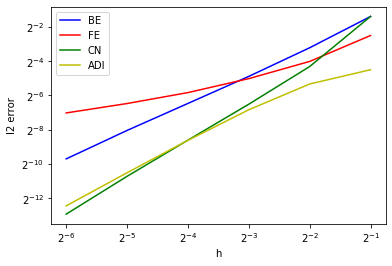
\includegraphics[width=1\textwidth]{immagini/validation_log-error}\caption{\label{fig:Err_par}Plot of the error \ref{eq:err_l2} in logarithmic
scale.}
\end{figure}

\begin{figure}[H]
\noindent \centering{}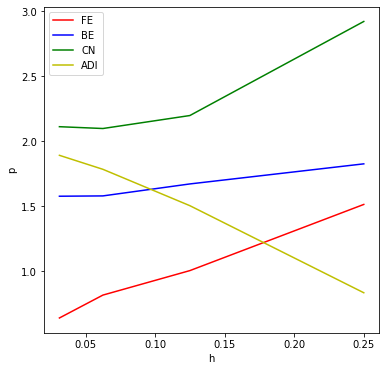
\includegraphics[width=1\textwidth]{immagini/validation_r}\caption{\label{fig:Conv_rate_par}Plot of the convergence rates \ref{eq:conv_rate}
of Forward Euler (FE), Backward Euler (BE), Crank-Nicolson (CN), Alternating
direction implicit method (ADI).}
\end{figure}
As expected, Forward Euler and Backward Euler have a lower convergence
rate than ADI and Crank-Nicolson. In this particular case, BE has
$p\approx1.5$ that is higher than what we expect. This is due, probably,
to a particularly simple manufactured solution. While both CN and
ADI reach $p=2$ with about $h\approx0.05$.

\section{The hyperbolic dynamics\label{sec:Hyperbolic-dynamic}}

The equation $\ref{eq:vick}$ has a drawback (the same of the Fourier
equation): \textit{the speed of information propagation is faster
than the speed of light in vacuum}. In 2010, Amadori, Boccabella and
Natalini \cite{amadori_one_2010} to overcome this problem proposed
a new 1-D spatial version of the replicator equation with finite speed
of propagation (similarly to Cattaneo works for the Fourier equation):
\begin{equation}
\begin{cases}
\frac{\partial n_{\ell}}{\partial t} & =-\frac{\partial\omega_{\ell}}{\partial x}+n_{\ell}\left[\frac{\mathbf{e_{\ell}}^{T}A\,\mathbf{n}}{N}-\frac{\mathbf{n}^{T}A\,\mathbf{n}}{N^{2}}\right]\\
\tau\frac{\partial\omega_{\ell}}{\partial t} & =-\lambda_{\ell}^{2}\frac{\partial n_{i}}{\partial x}-\omega_{\ell}
\end{cases}\qquad\ell=1,2.\label{eq:natal}
\end{equation}
Here $\mathbf{\omega_{\ell}}$ is the flux, $\tau$ is the relaxation
time and $\lambda_{\ell}$ is related to the dispersal rate. We extend
\ref{eq:natal} to two dimensions:
\begin{equation}
\begin{cases}
\frac{\partial n_{\ell}}{\partial t} & =-\left(\frac{\partial\varphi_{\ell}}{\partial x}+\frac{\partial\psi_{\ell}}{\partial y}\right)+n_{\ell}\left[\frac{\mathbf{e_{\ell}}^{T}A\,\mathbf{n}}{N}-\frac{\mathbf{n}^{T}A\,\mathbf{n}}{N^{2}}\right]\\
\tau\frac{\partial\varphi_{\ell}}{\partial t} & =-\lambda_{\ell}^{2}\frac{\partial n_{\ell}}{\partial x}-\varphi_{\ell}\\
\tau\frac{\partial\psi_{\ell}}{\partial t} & =-\lambda_{\ell}^{2}\frac{\partial n_{\ell}}{\partial y}-\psi_{\ell}
\end{cases}\qquad\ell=1,2\label{eq:2d_nat}
\end{equation}
 here $\varphi_{\ell}$ is the flux along $x$ and $\psi_{\ell}$
the one along $y$. In more dimensions and in a more compact form
the equation is:
\[
\begin{cases}
\frac{\partial n_{\ell}}{\partial t} & =-\bm{\nabla}\cdot\bm{\omega}_{\ell}+n_{\ell}\left[\frac{\mathbf{e_{\ell}}^{T}A\,\mathbf{n}}{N}-\frac{\mathbf{n}^{T}A\,\mathbf{n}}{N^{2}}\right]\\
\tau\frac{\partial\bm{\omega}_{\ell}}{\partial t} & =-\lambda_{\ell}^{2}\nabla n_{\ell}-\bm{\omega}_{\ell}
\end{cases}\qquad\ell=1,2
\]
whe\textcolor{black}{re $\bm{\omega}_{\ell}=\left(\begin{array}{c}
\varphi_{\ell}\\
\psi_{\ell}
\end{array}\right)$ is the flux vector of the population $\ell$.}

\textcolor{black}{We can study the evolution of the total number density.
Using the source term, i.e. \ref{eq:source}, we have from the first
pair of equations:
\begin{align*}
\frac{\partial N}{\partial t} & =\frac{\partial n_{1}}{\partial t}+\frac{\partial n_{2}}{\partial t}=\\
 & =-\left(\frac{\partial\varphi_{1}}{\partial x}+\frac{\partial\psi_{1}}{\partial y}\right)-\left(\frac{\partial\varphi_{2}}{\partial x}+\frac{\partial\psi_{2}}{\partial y}\right)-g\left(\mathbf{n}\right)+g\left(\mathbf{n}\right)\\
 & =-\frac{\partial}{\partial x}\left(\varphi_{1}+\varphi_{2}\right)-\frac{\partial}{\partial y}\left(\psi_{1}+\psi_{2}\right)=-\bm{\nabla}\cdot\left(\bm{\omega}_{1}+\bm{\omega}_{2}\right)
\end{align*}
The total population living in $\left(0,L_{x}\right)\times\left(0,L_{y}\right)$
is given by:
\begin{equation}
\tilde{N}\left(t\right)\coloneqq\intop_{0}^{L_{y}}\intop_{0}^{L_{x}}N\left(\mathbf{x},t\right)dx\,dy\label{eq:N_tot}
\end{equation}
 and its variation in time is:
\begin{align}
\frac{d\tilde{N}\left(t\right)}{dt} & =\intop_{0}^{L_{y}}\intop_{0}^{L_{x}}\frac{\partial N}{\partial t}dx\,dy=-\intop_{0}^{L_{y}}\intop_{0}^{L_{x}}-\bm{\nabla}\cdot\left(\bm{\omega}_{1}+\bm{\omega}_{2}\right)dx\,dy.\label{eq:N_nat}
\end{align}
This is essentially the same of \ref{eq:N_vick}, i.e. $N$ can only
change by the flux of player across the boundary of the considered
region.}

We will study the dynamics \ref{eq:2d_nat} on a two dimensional plane
$\left[0,L_{x}\right]\times\left[0,L_{y}\right]$ in a time interval
$\left[0,T\right]$ with the following initial conditions:
\begin{align*}
\begin{cases}
n_{1}\left(x,y,0\right) & =n_{1}^{0}\left(x,y\right)\\
\varphi_{1}\left(x,y,0\right) & =0\\
\psi_{1}\left(x,y,0\right) & =0\\
n_{2}\left(x,y,0\right) & =n_{2}^{0}\left(x,y\right)\\
\varphi_{2}\left(x,y,0\right) & =0\\
\psi_{2}\left(x,y,0\right) & =0
\end{cases}
\end{align*}
we choose zero value initial flux, but we consider three forms of
$n_{1}^{0}\left(x,y\right)$ and $n_{2}^{0}\left(x,y\right)$:
\begin{enumerate}
\item a random value between $0$ to $1$, i.e. for $\ell=1,2$:
\[
\forall x,y\quad n_{\ell}^{0}\left(x,y\right)=random\left[0,1\right];
\]
\item a single defector in a sea of cooperators, i.e. for the cooperators:
\[
n_{1}^{0}\left(x,y\right)=\begin{cases}
1 & if\ x\neq\frac{L_{x}}{2}\ or\ y\neq\frac{L_{y}}{2}\\
0 & otherwise
\end{cases}
\]
 and for the defectors:
\[
n_{2}^{0}\left(x,y\right)=\begin{cases}
1 & if\ x=\frac{L_{x}}{2}\ and\ y=\frac{L_{y}}{2}\\
0 & otherwise
\end{cases};
\]
\item a delta-type of defectors, rather the defectors are distributed along
a segment surrounded by cooperators, i.e.:
\begin{align*}
n_{1}^{0}\left(x,y\right) & =\begin{cases}
1 & if\ x\neq\frac{L_{x}}{2}\\
0 & otherwise
\end{cases}\\
n_{2}^{0}\left(x,y\right) & =\begin{cases}
1 & if\ x=\frac{L_{x}}{2}\\
0 & otherwise
\end{cases}
\end{align*}
\end{enumerate}
As done in section \ref{sec:Parabolic-dynamic}, the boundary conditions
are always zero, i.e. for $\ell=1,2$:
\begin{align*}
n_{\ell}\left(0,0,t\right) & =n_{\ell}\left(0,L_{y},t\right)=n_{\ell}\left(L_{x},0,t\right)=n_{\ell}\left(L_{x},L_{y},t\right)=0\quad\forall t\in\left[0,T\right]\\
\varphi_{\ell}\left(0,0,t\right) & =\varphi_{\ell}\left(0,L_{y},t\right)=\varphi_{\ell}\left(L_{x},0,t\right)=\varphi_{\ell}\left(L_{x},L_{y},t\right)=0\quad\forall t\in\left[0,T\right]\\
\psi_{\ell}\left(0,0,t\right) & =\psi_{\ell}\left(0,L_{y},t\right)=\psi_{\ell}\left(L_{x},0,t\right)=\psi_{\ell}\left(L_{x},L_{y},t\right)=0\quad\forall t\in\left[0,T\right]
\end{align*}

Moreover, we can see that equation \ref{eq:2d_nat} is a hyperbolic
PDE, so we use and compare two finite-difference methods, namely the
Lax method and the Lax-Wendroff method (for more details \cite{ames_numerical_1992,press_numerical_2007,pang_introduction_2006,thomas1995numerical,thomas1999numerical}).

Moreover, we can see that equation \ref{eq:2d_nat} is a hyperbolic
PDE. We use two finite difference algorithms:
\begin{itemize}
\item Lax;
\item Lax-Wendroff.
\end{itemize}

\subsection{Lax}

Lax method \cite{press_numerical_2007} is one of the most simple
finite difference explicit algorithm. Preserving the notation adopted
above, the first equation of the system can be written:

\begin{align*}
\frac{1}{\Delta t}\left\{ \left(n_{\ell}\right)_{i,j}^{k+1}-\frac{1}{4}\left[\left(n_{\ell}\right)_{i+1,j}^{k}\right.\right.\\
\left.\left.+\left(n_{\ell}\right)_{i-1,j}^{k}+\left(n_{\ell}\right)_{i,j+1}^{k}+\left(n_{\ell}\right)_{i,j-1}^{k}\right]\right\}  & =-\frac{\left(\varphi_{\ell}\right)_{i+1,j}^{k}-\left(\varphi_{\ell}\right)_{i-1,j}^{k}}{\Delta x}\\
 & -\frac{\left(\psi_{\ell}\right)_{i,j+1}^{k}-\left(\psi_{\ell}\right)_{i,j-1}^{k}}{\Delta y}\\
 & +\left(-1\right)^{\ell}\frac{\left(n_{1}\right)_{i.j}^{k}\left(n_{2}\right)_{i,j}^{k}}{\left(\left(n_{1}\right)_{i.j}^{k}+\left(n_{2}\right)_{i.j}^{k}\right)^{2}}\left(b-1\right)\left(n_{1}\right)_{i.j}^{k}
\end{align*}
 the second equation becomes:
\begin{align*}
\tau\frac{\left(\varphi_{\ell}\right)_{i,j}^{k+1}-\frac{1}{2}\left[\left(\varphi_{\ell}\right)_{i+1,j}^{k}+\left(\varphi_{\ell}\right)_{i-1,j}^{k}\right]}{\Delta t}= & -\left(\varphi_{\ell}\right)_{i,j}^{k}\\
 & -\lambda_{\ell}^{2}\frac{\left(n_{\ell}\right)_{i+1,j}^{k}-\left(n_{\ell}\right)_{i-1,j}^{k}}{\Delta x}
\end{align*}
 and for the third equation we have:
\begin{align*}
\tau\frac{\left(\psi_{\ell}\right)_{i,j}^{k+1}-\frac{1}{2}\left[+\left(\psi_{\ell}\right)_{i,j+1}^{k}+\left(\psi_{\ell}\right)_{i,j-1}^{k}\right]}{\Delta t} & =-\left(\psi_{\ell}\right)_{i,j}^{k}\\
 & -\lambda_{\ell}^{2}\frac{\left(n_{\ell}\right)_{i,j+1}^{k}-\left(n_{\ell}\right)_{i,j-1}^{k}}{\Delta y}.
\end{align*}
And so, we have the updating formulae:
\begin{align}
\left(n_{\ell}\right)_{i,j}^{k+1}= & \frac{1}{4}\left[\left(n_{\ell}\right)_{i+1,j}^{k}+\left(n_{\ell}\right)_{i-1,j}^{k}+\left(n_{\ell}\right)_{i,j+1}^{k}+\left(n_{\ell}\right)_{i,j-1}^{k}\right]\nonumber \\
 & -\Delta t\frac{\left(\varphi_{\ell}\right)_{i+1,j}^{k}-\left(\varphi_{\ell}\right)_{i-1,j}^{k}}{\Delta x}\nonumber \\
 & -\Delta t\frac{\left(\psi_{\ell}\right)_{i,j+1}^{k}-\left(\psi_{\ell}\right)_{i,j-1}^{k}}{\Delta y}\nonumber \\
 & +\Delta t\left(-1\right)^{\ell}\frac{\left(n_{1}\right)_{i.j}^{k}\left(n_{2}\right)_{i,j}^{k}}{\left(\left(n_{1}\right)_{i.j}^{k}+\left(n_{2}\right)_{i.j}^{k}\right)^{2}}\left(b-1\right)\left(n_{1}\right)_{i.j}^{k}\nonumber \\
\left(\varphi_{\ell}\right)_{i,j}^{k+1}= & \frac{1}{2}\left[\left(\varphi_{\ell}\right)_{i+1,j}^{k}+\left(\omega_{\ell}\right)_{i-1,j}^{k}\right]\nonumber \\
 & -\frac{\lambda_{\ell}^{2}}{\tau}\frac{\left(n_{\ell}\right)_{i+1,j}^{k}-\left(n_{\ell}\right)_{i-1,j}^{k}}{\Delta x}\nonumber \\
 & -\frac{\left(\varphi_{\ell}\right)_{i,j}^{k}}{\tau}.\nonumber \\
\left(\psi_{\ell}\right)_{i,j}^{k+1}= & \frac{1}{2}\left[\left(\psi_{\ell}\right)_{i,j+1}^{k}+\left(\psi_{\ell}\right)_{i,j-1}^{k}\right]\nonumber \\
 & -\frac{\lambda_{\ell}^{2}}{\tau}\frac{\left(n_{\ell}\right)_{i,j+1}^{k}-\left(n_{\ell}\right)_{i,j-1}^{k}}{\Delta y}\nonumber \\
 & -\frac{\left(\psi_{\ell}\right)_{i,j}^{k}}{\tau}.\label{eq:lax}
\end{align}


\subsection{Lax-Wendroff }

In 1960, Lax and Wendroff developed in their paper \cite{lax_systems_1960}
an explicit numerical scheme for hyperbolic PDE, based on the central
differences in space and second order Taylor expansion in time. In
two spatial dimension:
\begin{align*}
\left(n_{\ell}\right)_{i,j}^{k+1}= & \left(n_{\ell}\right)_{i,j}^{k}\\
 & -\frac{1}{2}\frac{\Delta t}{\Delta x}\left(\left(\varphi_{\ell}\right)_{i+1,j}^{k}-\left(\varphi_{\ell}\right)_{i-1,j}^{k}\right)\\
 & -\frac{1}{2}\frac{\Delta t}{\Delta y}\left(\left(\psi_{\ell}\right)_{i,j+1}^{k}-\left(\psi_{\ell}\right)_{i,j-1}^{k}\right)\\
 & +\frac{\Delta t^{2}}{2\Delta x^{2}}\left(\left(\varphi_{\ell}\right)_{i+1,j}^{k}-2\left(\varphi_{\ell}\right)_{i,j}^{k}+\left(\varphi_{\ell}\right)_{i-1,j}^{k}\right)\\
 & +\frac{\Delta t^{2}}{2\Delta y^{2}}\left(\left(\psi_{\ell}\right)_{i,j+1}^{k}-2\left(\psi_{\ell}\right)_{i,j}^{k}+\left(\psi_{\ell}\right)_{i,j-1}^{k}\right)\\
 & +\Delta t\left(-1\right)^{\ell}\frac{\left(n_{1}\right)_{i.j}^{k}\left(n_{2}\right)_{i,j}^{k}}{\left(\left(n_{1}\right)_{i.j}^{k}+\left(n_{2}\right)_{i.j}^{k}\right)^{2}}\left(b-1\right)\left(n_{1}\right)_{i.j}^{k}\\
\left(\varphi_{\ell}\right)_{i,j}^{k+1}= & \left(\varphi_{\ell}\right)_{i,j}^{k}\\
 & -\frac{\lambda_{\ell}^{2}}{2\tau}\frac{\Delta t}{\Delta x}\left(\left(n_{\ell}\right)_{i+1,j}^{k}-\left(n_{\ell}\right)_{i-1,j}^{k}\right)\\
 & +\frac{\lambda_{\ell}^{4}}{2\tau^{2}}\frac{\Delta t^{2}}{\Delta x^{2}}\left(\left(n_{\ell}\right)_{i+1,j}^{k}-2\left(n_{\ell}\right)_{i,j}^{k}+\left(n_{\ell}\right)_{i-1,j}^{k}\right)\\
 & -\frac{\left(\varphi_{\ell}\right)_{i,j}^{k}}{\tau}\\
\left(\psi_{\ell}\right)_{i,j}^{k+1}= & \left(\psi_{\ell}\right)_{i,j}^{k}\\
 & -\frac{\lambda_{\ell}^{2}}{2\tau}\frac{\Delta t}{\Delta y}\left(\left(n_{\ell}\right)_{i,j+1}^{k}-\left(n_{\ell}\right)_{i,j-1}^{k}\right)\\
 & +\frac{\lambda_{\ell}^{4}}{2\tau^{2}}\frac{\Delta t^{2}}{\Delta y^{2}}\left(\left(n_{\ell}\right)_{i,j+1}^{k}-2\left(n_{\ell}\right)_{i,j}^{k}+\left(n_{\ell}\right)_{i,j-1}^{k}\right)\\
 & -\frac{\left(\psi_{\ell}\right)_{i,j}^{k}}{\tau}
\end{align*}


\subsection{A drawback}

Finite difference methods have a big limit, well described by Godunov's
theorem \cite{Godunov54,Godunov59}:
\begin{thm}
Assume a continuum problem described by a PDE is to be computed using
a numerical scheme based upon a uniform computational grid and a one-step,
constant step-size, $M$ grid points integration algorithm, either
implicit or explicit. Writing $x_{j}=j\Delta x$ and $t_{n}=n\Delta t$,
such a scheme can be described by:
\[
\varphi_{j}^{n+1}=\sum\limits _{m}^{M}{\gamma_{m}\varphi_{j+m}^{n}}
\]
Then the above scheme is monotonicity preserving, i.e.:
\[
if\quad\varphi_{j+1}^{n}\geq\varphi_{j}^{n}\quad\forall j\Rightarrow\varphi_{j+1}^{n+1}\geq\varphi_{j}^{n+1}\quad\forall j
\]
 if and only if: 

\[
\gamma_{m}\ge0,\quad\forall m
\]
\end{thm}

In other words, it establishes that a monotone behaviour of a numerical
solution cannot be assured for linear finite-difference methods with
more than first-order accuracy (for more details \cite{tryggvason_lecture_2017,thirumgam_numerical_2012}).
This problem is clear in fig \ref{fig:oscill_example}, where we compared
the Lax and Lax-Wendroff methods for our one-dimensional problem.

\begin{figure}
\subfloat[]{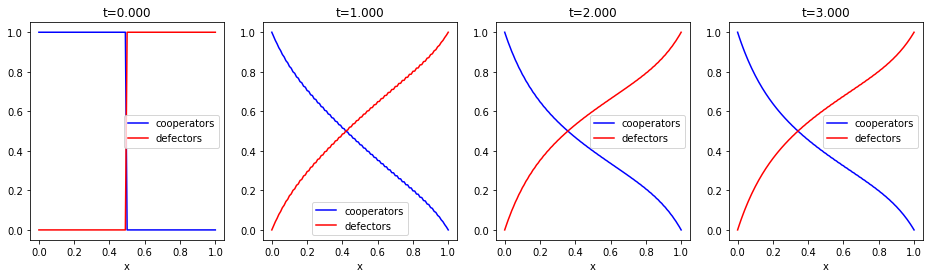
\includegraphics[width=1\textwidth]{immagini/lax_example}

}

\subfloat[]{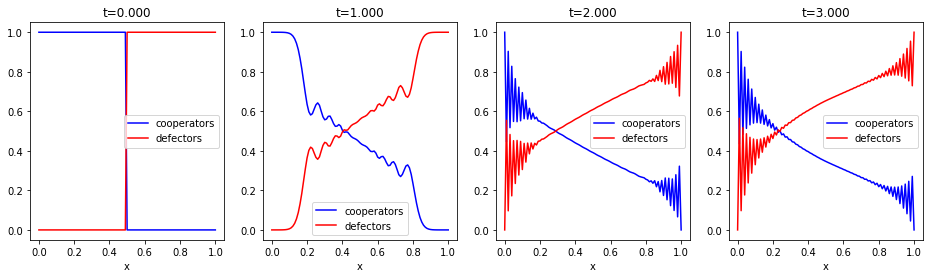
\includegraphics[width=1\textwidth]{immagini/l-w_example}

}

\caption{\label{fig:oscill_example}Numerical solution of $n_{1}$ and $n_{2}$
of \ref{eq:natal} with $T=3$ and $L_{x}=1.0$, setting $\lambda=0.3$,
$\tau=0.8$ and $b=1.85$, with Lax method (A) and Lax-Wendroff one
(B). The boundary condition are $n_{1}(0,t)=1$, $n_{1}(L_{x},t)=0$,
$n_{2}(0,t)=0$ and $n_{2}(L_{x},t)=1$.}

\end{figure}

As expected, the solutions of the Lax-Wendroff are not monotonic.
One way to overcome this limit is to use \textit{artificial viscosity}
\cite{vonneumann_method_1950,Biringen2011}. In practice, a term of
artificial dissipation is added to smooth the numerical solutions.
Considering \ref{eq:natal}, this term is written as:
\begin{align*}
q_{n_{\ell}} & =\mu_{n}\left(\left(n_{\ell}\right)_{i+1}^{k}-2\left(n_{\ell}\right)_{i}^{k}+\left(n_{\ell}\right)_{i-1}^{k}\right)\\
q_{\varphi_{\ell}} & =\mu_{\varphi}\left(\left(\varphi_{\ell}\right)_{i+1}^{k}-2\left(\varphi_{\ell}\right)_{i}^{k}+\left(\varphi_{\ell}\right)_{i-1}^{k}\right)\\
q_{\psi_{\ell}} & =\mu_{\psi}\left(\left(\psi_{\ell}\right)_{i+1}^{k}-2\left(\psi_{\ell}\right)_{i}^{k}+\left(\psi_{\ell}\right)_{i-1}^{k}\right)
\end{align*}

where $\mu_{n}$, $\mu_{\varphi}$ and $\mu_{\psi}$ are two constants
in $\left[0,1\right]$. How the artificial viscosity modifies the
results are quite controversial, but it has been used often. We can
see the reason why in fig \ref{fig:art_visc_example}.

\begin{figure}
\subfloat[]{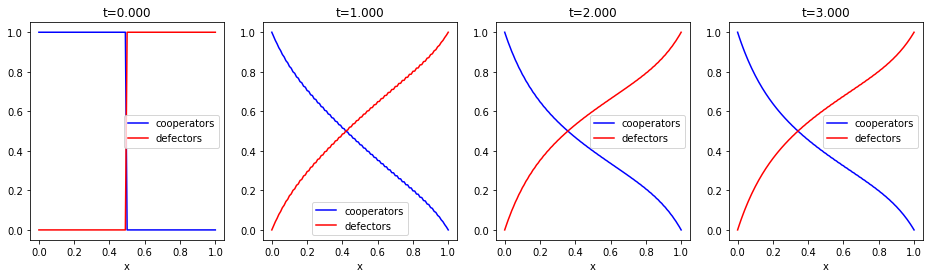
\includegraphics[width=1\textwidth]{immagini/lax_example}

}

\subfloat[]{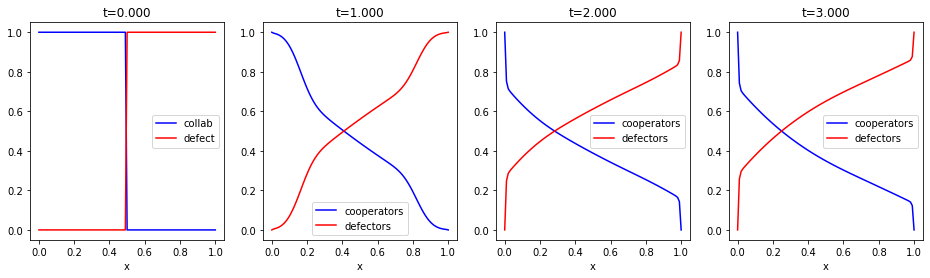
\includegraphics[width=1\textwidth]{immagini/l-w-av_example}

}

\caption{\label{fig:art_visc_example}Numerical solution of $n_{1}$ and $n_{2}$
of \ref{eq:natal} with $T=3$ and $L_{x}=1.0$, setting $\lambda=0.3$,
$\tau=0.8$ and $b=1.85$, with Lax method (A) and Lax-Wendroff one
with artificial viscosity with $\mu_{n}=\mu_{\omega}=0.05$ (B). The
boundary condition are $n_{1}(0,t)=1$, $n_{1}(L_{x},t)=0$, $n_{2}(0,t)=0$
and $n_{2}(L_{x},t)=1$.}
\end{figure}

In our work, we choose $\mu_{n}$, $\mu_{\varphi}$ and $\mu_{\psi}$
empirically.

\subsection{Verification}

Now, we can verify the code, as seen above. The chosen \textit{manufactured
solutions} for the hyperbolic model are:
\begin{align*}
n_{1ex}\left(x,y,t\right) & =5e^{\text{\textminus}2\frac{t}{\tau}}\left(x-L_{x}\right)\left(y-L_{y}\right),\\
\varphi_{1ex}\left(x,y,t\right) & =1,\\
\psi_{1ex}\left(x,y,t\right) & =1,\\
n_{2ex}\left(x,y,t\right) & =e^{\text{\textminus}2\frac{t}{\tau}}\left(x-L_{x}\right)\left(y-L_{y}\right),\\
\varphi_{2ex}\left(x,y,t\right) & =1,\\
\psi_{2ex}\left(x,y,t\right) & =1.
\end{align*}

And so, inserting them in \ref{eq:2d_nat}, the source terms are (computed
with \textit{sympy}):

\begin{align*}
f_{n_{1}}= & 0.069\bar{4}\left(x-L_{x}\right)\left(y-L_{y}\right)e^{\text{\textminus}2\frac{t}{\tau}}-\frac{2}{\tau}(5x-5L_{x})(y-L_{y})e^{\text{\textminus}2\frac{t}{\tau}}\\
f_{\varphi_{1}}= & \lambda^{2}e^{\text{\textminus}2\frac{t}{\tau}}(5y-5L_{y})+1\\
f_{\psi_{1}}= & \lambda^{2}e^{\text{\textminus}2\frac{t}{\tau}}(5x-5L_{x})+1\\
f_{n_{2}}= & -0.069\bar{4}\left(x-L_{x}\right)\left(y-L_{y}\right)e^{\text{\textminus}2\frac{t}{\tau}}-\frac{2}{\tau}(x-L_{x})(y-L_{y})e^{\text{\textminus}2\frac{t}{\tau}}\\
f_{\varphi_{2}}= & \lambda^{2}e^{\text{\textminus}2\frac{t}{\tau}}(y-L_{y})+1\\
f_{\psi_{2}}= & \lambda^{2}e^{\text{\textminus}2\frac{t}{\tau}}(x-L_{x})+1
\end{align*}

Then, we can compute the $\ell^{2}$ error:
\begin{align}
E_{n_{1}} & =\sqrt{\Delta x\:\Delta y\:\sum_{j=0}^{N_{y}}\:\sum_{i=0}^{N_{x}}\left(n_{1ex}\left(i\cdot dx,\,j\cdot dy,\,T\right)-\left(n_{1}\right)_{i,j}^{N_{t}}\right)},\label{eq:err_l2_hyp}\\
E_{\varphi_{1}} & =\sqrt{\Delta x\:\Delta y\:\sum_{j=0}^{N_{y}}\:\sum_{i=0}^{N_{x}}\left(\varphi_{1ex}\left(i\cdot dx,\,j\cdot dy,\,T\right)-\left(\varphi_{1}\right)_{i,j}^{N_{t}}\right)},\nonumber \\
E_{\psi_{1}} & =\sqrt{\Delta x\:\Delta y\:\sum_{j=0}^{N_{y}}\:\sum_{i=0}^{N_{x}}\left(\psi_{1ex}\left(i\cdot dx,\,j\cdot dy,\,T\right)-\left(\psi_{1}\right)_{i,j}^{N_{t}}\right)},\nonumber \\
E_{n_{2}} & =\sqrt{\Delta x\:\Delta y\:\sum_{j=0}^{N_{y}}\:\sum_{i=0}^{N_{x}}\left(n_{2ex}\left(i\cdot dx,\,j\cdot dy,\,T\right)-\left(n_{2}\right)_{i,j}^{N_{t}}\right)},\nonumber \\
E_{\varphi_{2}} & =\sqrt{\Delta x\:\Delta y\:\sum_{j=0}^{N_{y}}\:\sum_{i=0}^{N_{x}}\left(\varphi_{2ex}\left(i\cdot dx,\,j\cdot dy,\,T\right)-\left(\varphi_{2}\right)_{i,j}^{N_{t}}\right)},\nonumber \\
E_{\psi_{2}} & =\sqrt{\Delta x\:\Delta y\:\sum_{j=0}^{N_{y}}\:\sum_{i=0}^{N_{x}}\left(\psi_{2ex}\left(i\cdot dx,\,j\cdot dy,\,T\right)-\left(\psi_{2}\right)_{i,j}^{N_{t}}\right)}\nonumber 
\end{align}
 Now, we can plot the error (fig \ref{fig:Err_hyp}) and the convergence
rates (fig \ref{fig:Conv_rate_hyp}).

\begin{figure}[H]
\noindent \centering{}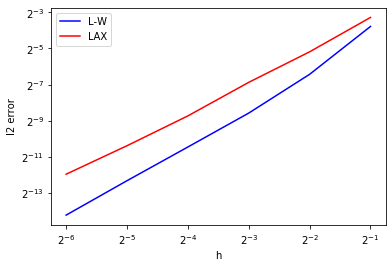
\includegraphics[width=1\textwidth]{immagini/validation_log-error_hyp}\caption{\foreignlanguage{english}{\label{fig:Err_hyp}Plot of the error \ref{eq:err_l2_hyp} in logarithmic
scale.}}
\end{figure}

\begin{figure}[H]
\noindent \centering{}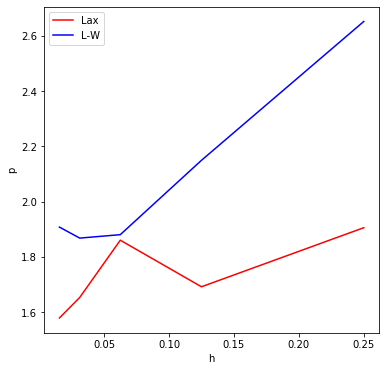
\includegraphics[width=1\textwidth]{immagini/validation_r_hyp}\caption{\foreignlanguage{english}{\label{fig:Conv_rate_hyp}Plot of the convergence rates \ref{eq:conv_rate}
of Lax method and Lax-Wendroff method (L-W).}}
\end{figure}

We can observe that (after some fluctuations), the Lax-Wendroff method
converges to $p=2$, while the Lax one converges to smaller $p$.

\section{The simulations\label{sec:The-simulations}}

We solve the parabolic model \ref{eq:vick} and the hyperbolic model
\ref{eq:2d_nat} with the Crank-Nicolson for the former and the Lax-Wendroff
for the latter. As anticipated, we choose three different initial
conditions:
\begin{enumerate}
\item random spatial distribution of cooperators and defectors;
\item a single defector in a sea of cooperators;
\item a delta-type of defectors surrounded by cooperators.
\end{enumerate}

\subsection{Random initial condition}

In this simulation we assume an initial random distribution of cooperators
and defectors (fig \ref{fig:rand}). 

\begin{figure}
\subfloat[]{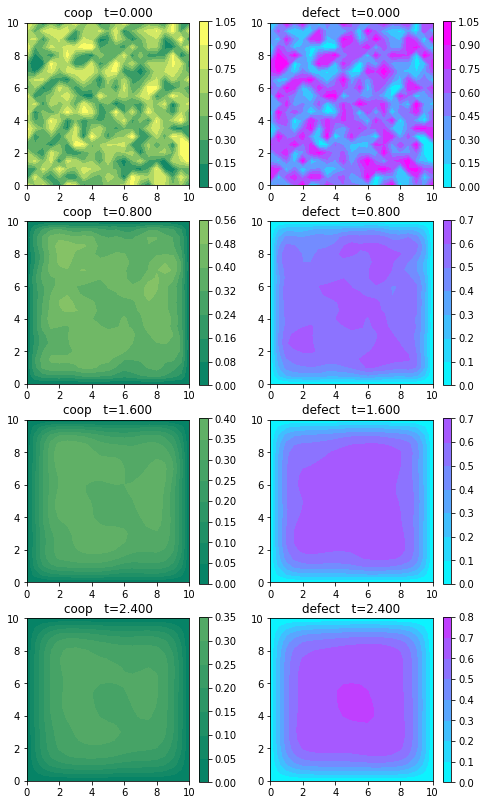
\includegraphics[width=0.5\textwidth]{immagini/CN-rand}

}\subfloat[]{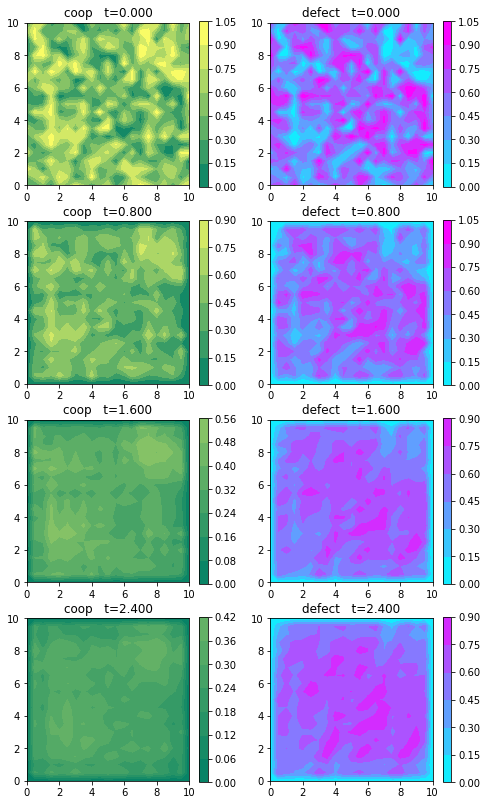
\includegraphics[width=0.5\textwidth]{immagini/l-w-rand}

}\caption{\label{fig:rand}Numerical solution of $n_{1}$ and $n_{2}$ in $T=2.4$
and $L_{x}=L_{y}=10$ of parabolic model \ref{eq:vick} using Crank-Nicolson
with $D=0.25$ (A) and hyperbolic model \ref{eq:2d_nat} using Lax-Wendroff
with artificial viscosity with $\mu_{n}=\mu_{\varphi}=\mu_{\psi}=0.001$,
$\lambda=0.5$ and $\tau=0.9$ (B). For both the methods we set $N_{x}=N_{y}=20$,
$dt=0.01$ and $b=1.85$.}
\end{figure}


\subsection{One defector in a sea of cooperators}

Second, we study the two equations setting at the starting time the
defectors in a single central point (fig \ref{fig:onedef}). 

\begin{figure}
\subfloat[]{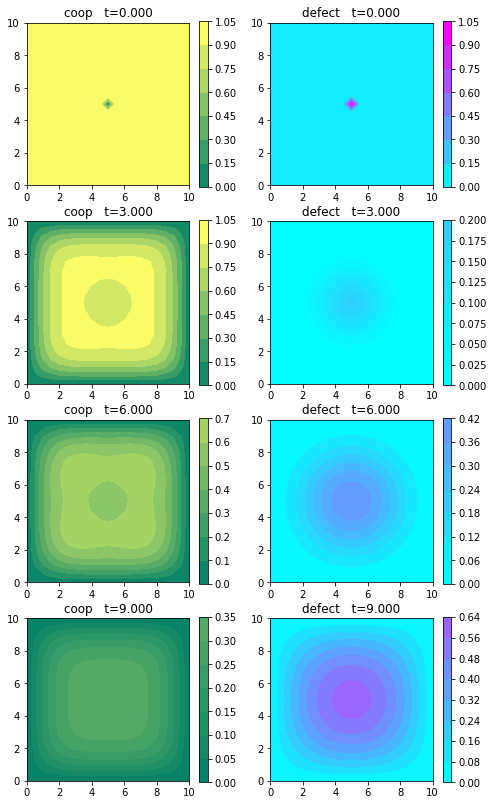
\includegraphics[width=0.5\textwidth]{immagini/CN-onedef}

}\subfloat[]{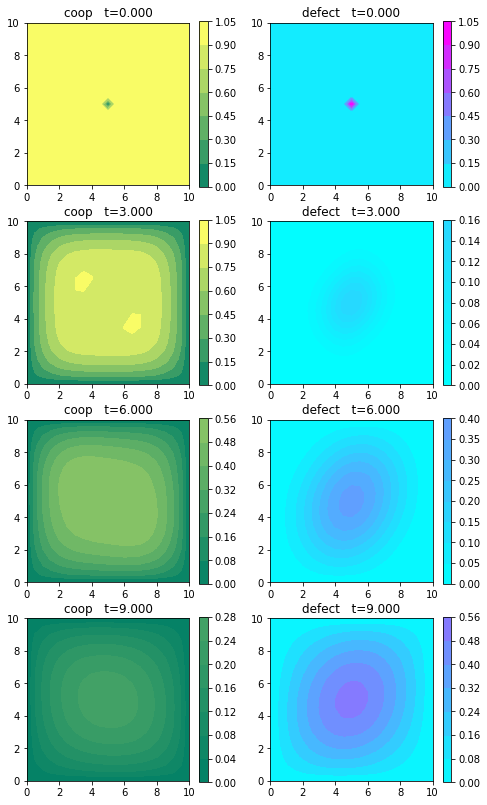
\includegraphics[width=0.5\textwidth]{immagini/l-w-onedef}

}

\caption{\label{fig:onedef}Numerical solution of $n_{1}$ and $n_{2}$ in
$T=9$ and $L_{x}=L_{y}=10$ of parabolic model \ref{eq:vick} using
Crank-Nicolson with $D=0.25$ (A) and hyperbolic model \ref{eq:2d_nat}
using Lax-Wendroff with artificial viscosity with $\mu_{n}=\mu_{\varphi}=\mu_{\psi}=0.001$,
$\lambda=0.5$ and $\tau=0.9$ (B). For both the methods we set $N_{x}=N_{y}=20$,
$dt=0.01$ and $b=1.85$.}
\end{figure}


\subsection{Delta initial condition}

Finally, we analyse the two models, arranging the defectors in delta-type
function in the space surrounded by the cooperators, at the initial
time (fig \ref{fig:delta}). 

\begin{figure}
\subfloat[]{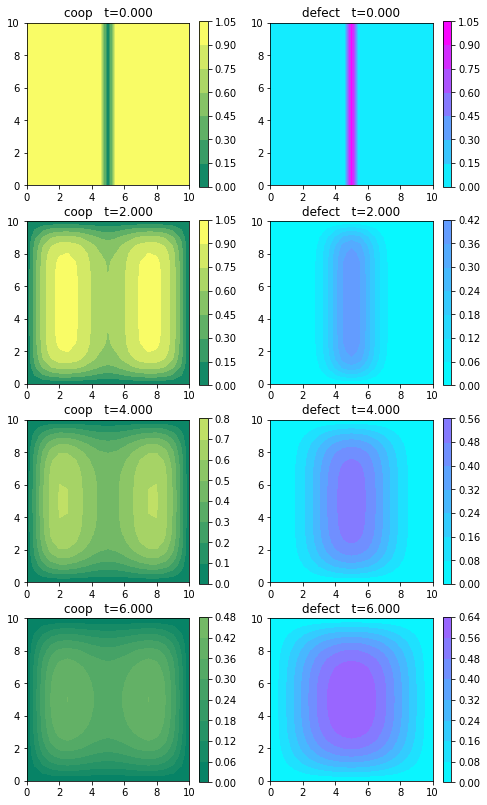
\includegraphics[width=0.5\textwidth]{immagini/CN-delta}

}\subfloat[]{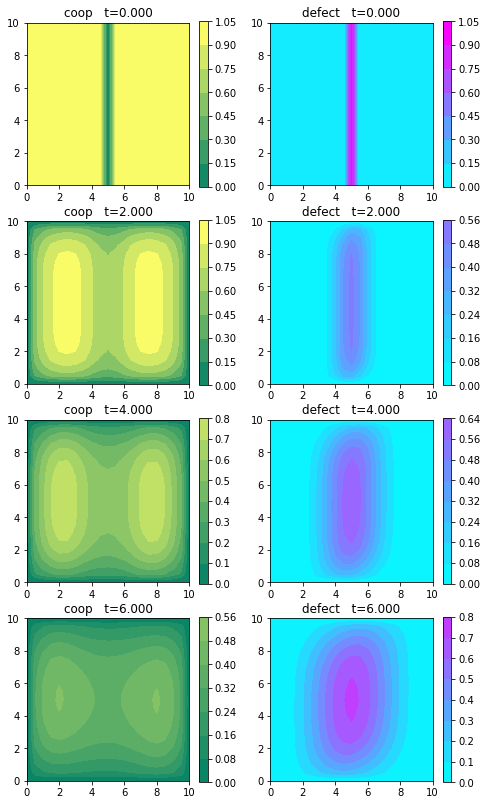
\includegraphics[width=0.5\textwidth]{immagini/l-w-delta}

}

\caption{\label{fig:delta}Numerical solution of $n_{1}$ and $n_{2}$ in $T=6$
and $L_{x}=L_{y}=10$ of parabolic model \ref{eq:vick} using Crank-Nicolson
with $D=0.25$ (A) and hyperbolic model \ref{eq:2d_nat} using Lax-Wendroff
with artificial viscosity with $\mu_{n}=\mu_{\varphi}=\mu_{\psi}=0.005$,
$\lambda=0.5$ and $\tau=0.9$ (B). For both the methods we set $N_{x}=N_{y}=20$,
$dt=0.01$ and $b=1.85$.}
\end{figure}


\subsection{Phase diagram and conclusion}

In brief, we can see that the evolution in the parabolic and hyperbolic
models is quite similar, and the defectors invade the whole of the
space and the population of cooperators becomes extinct. The hyperbolic
model needs more time to diffuse the population, but this is what
we expect because a limited speed is explicitly requested.

Now we want to try to understand the evolution as $b$ varies. Instead
of plotting the evolution of the populations in the space for each
value, we use the phase diagrams of the probability of a strategy
varying $b$. To obtain the probability of one of the strategies,
we must compute:
\[
p_{\ell}=\frac{\frac{1}{L_{x}L_{y}}\int_{0}^{L_{X}}\int_{0}^{L_{y}}n_{i}(x,y,t)dxdy}{\frac{1}{L_{x}L_{y}}\int_{0}^{L_{X}}\int_{0}^{L_{y}}\sum_{j}n_{j}(x,y,t)dxdy}\qquad t\rightarrow+\infty
\]

\begin{figure}
\subfloat[]{

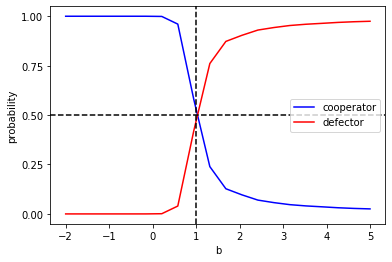
\includegraphics[width=0.5\textwidth]{immagini/CN_phase}

}\subfloat[]{

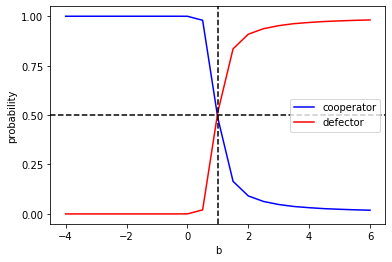
\includegraphics[width=0.5\textwidth]{immagini/l-w_phase}

}\caption{Phase diagrams of the parabolic model (A) and of the hyperbolic model
(B).}

\end{figure}

Not so surprisingly, we observe a phase transition when $b=1$. Recalling
the payoff matrix:
\[
A=\left(\begin{array}{cc}
R & S\\
T & P
\end{array}\right)=\left(\begin{array}{cc}
1 & 0\\
b & 0
\end{array}\right)
\]
 we have a phase transition when the payoff of the defection (i.e.
the temptation $T$) becomes higher than the one for the cooperation
(i.e. the reward $R$). 

\part{Discrete replicator and random walk}
\noindent \begin{flushright}
\textit{The theory of evolution is based on the }\\
\textit{struggle for life and the survival of the fittest. }\\
\textit{Yet cooperation is common between members of the same }\\
\textit{species and even between members of different species.}\\
\textit{ }Robert Axelrod
\par\end{flushright}

In this chapter, we propose a spatial discrete replicator equation.
We suppose the players as random walkers on a square lattice with
a sort of drift term due to the discrete replicator equation \cite{hofbauer_evolutionary_1998}:
\[
p_{\ell}^{k+1}=p_{\ell}^{k}\frac{c+\mathbf{e}_{\ell}^{T}A\mathbf{p}}{c+\mathbf{p}^{T}A\mathbf{p}}
\]
here c is a positive constant corresponding to the fitness in the
absence of interaction, $p_{\ell}^{k}$ is the frequency of strategy
$\ell$ at time $k$, and as in \ref{eq:replicator}, $\mathbf{e}_{\ell}^{T}A\mathbf{p}$
is the payoff of the focal player playing the strategy $\ell$ against
the population playing the mixed strategy $\mathbf{p}$, and $\mathbf{p}^{T}A\,\mathbf{p}$
is the payoff of the focal player playing the same mixed strategy
$\mathbf{p}$ of the population. Finally, we simulate it and discuss
the relation with the previous PDEs.

\section{A heuristic derivation\label{sec:A-heuristic-derivation} }

Consider a population of agents distributed on the cubic lattice $\mathbb{Z}^{m}$
and let $N^{k}=N^{k}\left(x\right)$ be the number (density) of agents
at site $x\in\mathbb{Z}^{m}$ at the time step $k$. Let $n_{\ell}^{k}\left(x\right)$
be the number of agents at $x$ playing strategy $\ell$ at time $k$,
so that, for games with two strategies, $\ell=1,2$ and $\sum_{\ell}n_{\ell}^{k}\left(x\right)=N^{k}\left(x\right)$.

Let $U\left(x\right)\subset\mathbb{Z}^{m}$ be the set of first neighbours
of $x$, i.e., $U\left(x\right)=\left\{ y\in\mathbb{Z}^{m}:\exists i\,\mid\,y_{i}=x_{i}\pm1\text{ and }y_{j}=x_{j}\text{ otherwise}\right\} $,
and define a random walk on the lattice by assigning uniform probability
to the jump from a point to each of its neighbours, i.e.:
\[
\mathbb{P}\left(y|x\right)=\begin{cases}
\frac{1}{2m} & \text{ if }y\in U(x)\\
0 & \text{otherwise}.
\end{cases}
\]
Here, we assume that two processes are active at each time step $k$
and lattice point $x$, and for every strategy $\ell$: 
\begin{itemize}
\item First, the population $n_{\ell}^{k}\left(x\right)$ of $\ell$-players
at each lattice point reproduces according to a discrete replicator
dynamics: the rate of growth of a subpopulation that plays $\ell$
is just its relative fitness, i.e. the ratio between the payoff of
the pure strategy against the population, and the average payoff of
the population. The number of offspring is therefore: 
\[
n_{\ell}^{k}\left(x\right)\frac{c+\frac{{\bf e}_{\ell}\cdot A{\bf n}^{k}\left(x\right)}{N^{k}\left(x\right)}}{c+\frac{{\bf n}^{k}\left(x\right)\cdot A{\bf n}^{k}\left(x\right)}{\left(N^{k}\left(x\right)\right)^{2}}},
\]
where, for two strategies, ${\bf n}^{k}\left(x\right)=\left(n_{1}^{k}\left(x\right),n_{2}^{k}\left(x\right)\right)$.
\item Then, the offspring remain at site $x$, but the parent population
migrates to the neighbouring lattice points according to the random
walk above. Hence, since the probability of remaining at the site
vanishes, the expected number of parents at site $x$ at time $k+1$
is given by:
\[
-n_{\ell}^{k}(x)+\sum_{y\in U(x)}\mathbb{P}\left(y|x\right)n_{\ell}^{k}\left(y\right)=\frac{1}{2m}\left(\sum_{y\in U(x)}\mathbb{P}\left(y|x\right)n_{\ell}^{k}\left(y\right)-2m\,n_{\ell}^{k}\left(x\right)\right),
\]
that accounts for the migration to site $x$ from its neighbours.
\end{itemize}
Hence, the population of $\ell$-agents at time $k+1$ at $x$ is:
\[
n_{\ell}^{k+1}(x)=\frac{1}{2m}\left(\sum_{y\in U(x)}\mathbb{P}\left(y|x\right)n_{\ell}^{k}\left(y\right)-2m\,n_{\ell}^{k}\left(x\right)\right)+n_{\ell}^{k}\left(x\right)\frac{c+\frac{{\bf e}_{\ell}\cdot A{\bf n}^{k}\left(x\right)}{N^{k}\left(x\right)}}{c+\frac{{\bf n}^{k}\left(x\right)\cdot A{\bf n}^{k}\left(x\right)}{\left(N^{k}\left(x\right)\right)^{2}}},
\]
which is our basic update rule for the population.

Introducing the Laplacian operator of the lattice by: 
\[
\mathcal{L}=B-2mI,
\]
where $I$ is the $K\times K$ identity matrix, $K$ is the number
of sites of the portion of the lattice we are working on, and $B$
is the adjacency matrix of the lattice, such that $B_{xy}=1$ only
if $y\in U(x)$, and zero otherwise, we can rewrite the update rule
as in terms of the Laplacian: 
\begin{equation}
n_{\ell}^{k+1}(x)=\frac{1}{2m}\sum_{y\in U(x)}\mathcal{L}_{xy}n_{\ell}^{k}\left(y\right)+n_{\ell}^{k}\left(x\right)\frac{c+\frac{{\bf e}_{\ell}\cdot A{\bf n}^{k}\left(x\right)}{N^{k}\left(x\right)}}{c+\frac{{\bf n}^{k}\left(x\right)\cdot A{\bf n}^{k}\left(x\right)}{\left(N^{k}\left(x\right)\right)^{2}}}.\label{eq:discr}
\end{equation}
For instance, in case of a 1-dimensional lattice, letting $x=i\in\mathbb{Z}$,
we have:
\[
n_{\ell}^{k+1}(i)=\frac{1}{2}(n_{\ell}^{k}(i+1)-2n_{\ell}^{k}(i)+n_{\ell}^{k}(i-1))+n_{\ell}^{k}(i)\frac{c+\frac{{\bf e}_{\ell}\cdot A{\bf n}^{k}(i)}{N^{k}(i)}}{c+\frac{{\bf n}^{k}\left(i\right)\cdot A{\bf n}^{k}(i)}{(N^{k}(i))^{2}}}.
\]


\section{The simulations\label{sec:The-simulations-1}}

We will study the dynamics \ref{eq:discr} on a two dimensional plane
$\left[0,L_{x}\right]\times\left[0,L_{y}\right]$ in a time interval
$\left[0,T\right]$, i.e. the equation for a two dimensional lattice
$x\equiv\left(i,j\right)\in\mathbb{Z}^{2}$ is:
\begin{align*}
n_{\ell}^{k+1}\left(i,j\right) & =\frac{1}{4}\left[\left(n_{\ell}^{k}\left(i+1,j\right)-2n_{\ell}^{k}\left(i,j\right)+n_{\ell}^{k}\left(i-1,j\right)\right)\right.\\
 & +\left.\left(n_{\ell}^{k}\left(i,j+1\right)-2n_{\ell}^{k}\left(i,j\right)+n_{\ell}^{k}\left(i,j-1\right)\right)\right]\\
 & +n_{\ell}^{k}(i,j)\frac{c+\frac{{\bf e}_{\ell}\cdot A{\bf n}^{k}(i,j)}{N^{k}(i,j)}}{c+\frac{{\bf n}^{k}\left(i,j\right)\cdot A{\bf n}^{k}(i,j)}{(N^{k}(i,j))^{2}}}
\end{align*}
Since it is discrete, performing simulations is much simpler. Then,
as done in the previous part, we consider three forms of $n_{1}^{0}\left(i,j\right)$
and $n_{2}^{0}\left(i,j\right)$:
\begin{enumerate}
\item a random value between $0$ to $1$, i.e. for $\ell=1,2$:
\[
\forall x,y\quad n_{\ell}^{0}\left(i,j\right)=random\left[0,1\right];
\]
\item a single defector in a sea of cooperators, i.e. for the cooperators:
\[
n_{1}^{0}\left(i,j\right)=\begin{cases}
1 & if\ i\neq\frac{L_{x}}{2}\ or\ j\neq\frac{L_{y}}{2}\\
0 & otherwise
\end{cases}
\]
 and for the defectors:
\[
n_{2}^{0}\left(i,j\right)=\begin{cases}
1 & if\ i=\frac{L_{x}}{2}\ and\ j=\frac{L_{y}}{2}\\
0 & otherwise
\end{cases};
\]
\item a delta-type of defectors surrounded by cooperators, i.e.:
\begin{align*}
n_{1}^{0}\left(i,j\right) & =\begin{cases}
1 & if\ i\neq\frac{L_{x}}{2}\\
0 & otherwise
\end{cases}\\
n_{2}^{0}\left(i,j\right) & =\begin{cases}
1 & if\ i=\frac{L_{x}}{2}\\
0 & otherwise
\end{cases}
\end{align*}
\end{enumerate}
We choose zero value boundary conditions, i.e. for $\ell=1,2$:
\[
n_{\ell}^{k}\left(0,0\right)=n_{\ell}^{k}\left(0,L_{y},t\right)=n_{\ell}^{k}\left(L_{x},0,t\right)=n_{\ell}^{k}\left(L_{x},L_{y},t\right)=0\quad\forall t\in\left[0,T\right].
\]


\subsection{Random initial condition}

We set a random initial position of cooperators and defectors in equal
proportion (fig \ref{fig:rand-1}). 

\begin{figure}
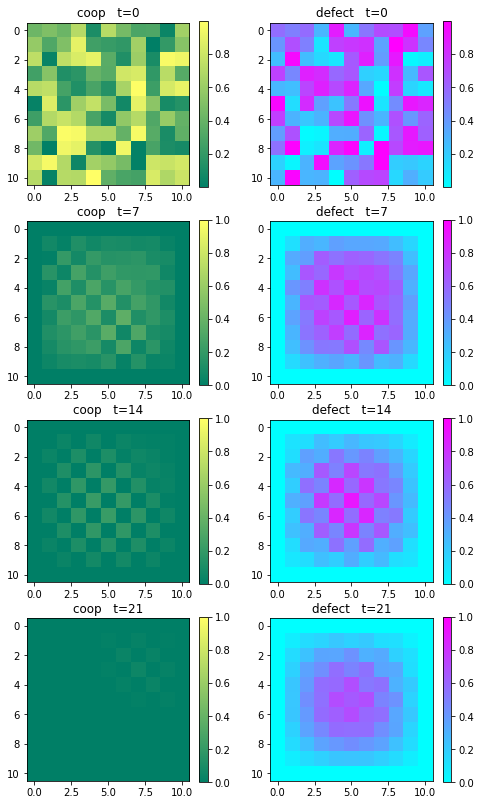
\includegraphics[width=0.75\textwidth]{immagini/discr-rand}

\caption{\label{fig:rand-1}Numerical solution of $n_{1}$ and $n_{2}$ in
$T=21$ and $L_{x}=L_{y}=10$ of \ref{eq:discr}. We set $b=1.85$.}
\end{figure}


\subsection{One defector in a sea of cooperators}

Secondly, we study the dynamics of the two population setting at the
starting time the defectors in a single central point surrounded by
the cooperators (fig \ref{fig:onedef-1}). 

\begin{figure}
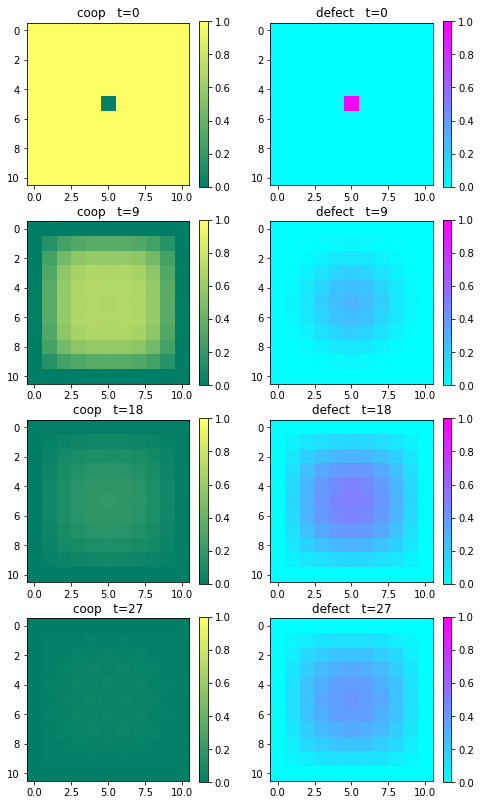
\includegraphics[width=0.75\textwidth]{immagini/discr-onedef}

\caption{\label{fig:onedef-1}Numerical solution of $n_{1}$ and $n_{2}$ in
$T=27$ and $L_{x}=L_{y}=10$ of \ref{eq:discr}. We set $b=1.85$.}
\end{figure}


\subsection{Delta initial condition}

Finally, we arrange the defectors in the delta-type function in the
space surrounded by the cooperators, at the initial time. We can see
the evolution below (fig \ref{fig:delta-1}). 

\begin{figure}
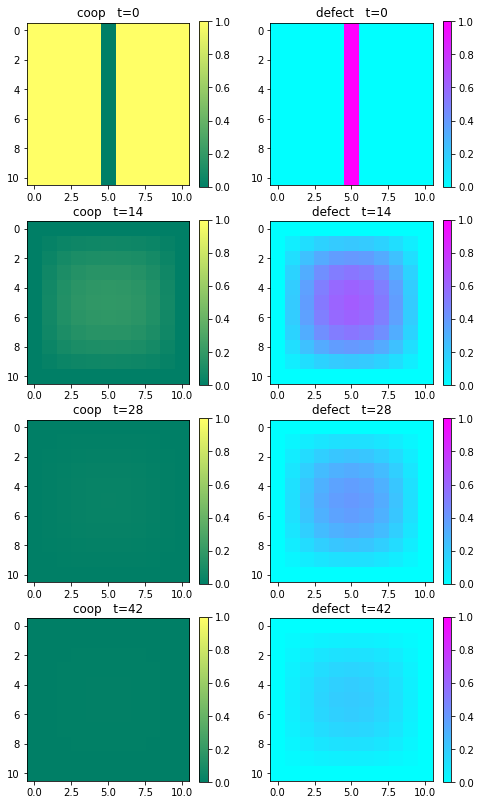
\includegraphics[width=0.75\textwidth]{immagini/discr-delta}

\caption{\label{fig:delta-1}Numerical solution of $n_{1}$ and $n_{2}$ in
$T=42$ and $L_{x}=L_{y}=10$ of \ref{eq:discr}.We set $b=1.85$.}
\end{figure}


\subsection{Phase diagram and conclusion}

The equation \ref{eq:discr} gives similar results to those we have
seen in the continuous models. In figure \ref{fig:N_tot}, we compare
the evolution of the total number $\tilde{N}$ in the three models,
for the 2-dimensional discrete model it is:
\[
\tilde{N}^{k}=\sum_{x\in\mathbb{Z}^{2}}N^{k}\left(x\right)
\]

\begin{figure}

\subfloat[]{

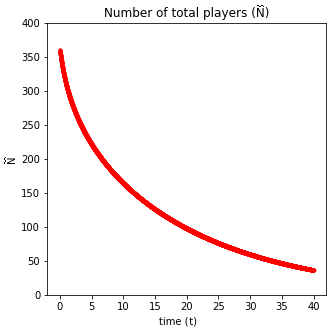
\includegraphics[width=0.33\textwidth]{immagini/Ntot_CN}} \subfloat[]{

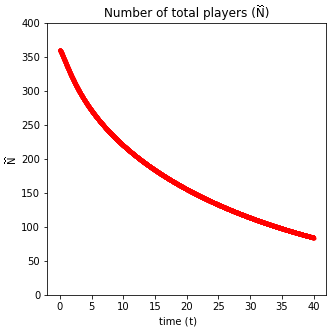
\includegraphics[width=0.33\textwidth]{immagini/Ntot_l-w}}\subfloat[]{

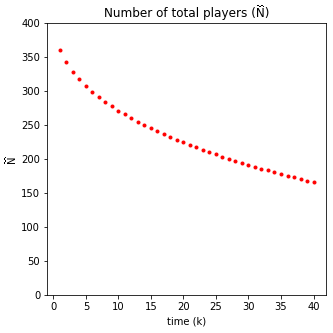
\includegraphics[width=0.33\textwidth]{immagini/Ntot_discr}

}\caption{\label{fig:N_tot} Evolution of the total density $\tilde{N}$ for
$T=40$ in the parabolic model (A), in the hyperbolic model (B) and
in the discrete model (C).}

\end{figure}

We can observe that in the three models $\tilde{N}$ decreases. In
the hyperbolic the speed of decrease is slower than the parabolic
and this is due to the ad-hoc flux, which forces the speed limit,
so there is no new information, but in the discrete one the decrease
is the slowest, with no assumption on the dispersal speed.

Moreover, as done for the continuous model, we want to try to understand
if there is a phase transition in the probability of a strategy varying
$b$. So, calling $\left|V\right|$ the number of nodes in the lattice,
the probability of the $\ell-th$ strategy is:
\[
p_{\ell}=\frac{\frac{1}{\left|V\right|}\sum_{\mathbf{x}:\forall\mathbf{x}\in\Gamma}n_{\ell}(\mathbf{x},t)}{\frac{1}{\left|V\right|}\sum_{j}\sum_{\mathbf{x}:\forall\mathbf{x}\in\Gamma}n_{j}(\mathbf{x},t)}\qquad t\rightarrow+\infty
\]

\begin{figure}
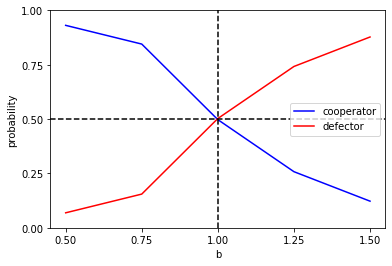
\includegraphics[width=0.75\textwidth]{immagini/discr_phase}\caption{\label{fig:Phase-diagrams}Phase diagrams of the parabolic model (A)
and of the hyperbolic model (B).}
\end{figure}

As for the continuous model, in fig \ref{fig:Phase-diagrams} we observe
a phase transition in $b=1$. This means that we have a phase transition
when the temptation $T$ becomes higher than the reward $R$.

\part{Voter model and reaction diffusion }
\noindent \begin{flushright}
\textit{I think that it is a relatively good approximation}\\
\textit{ to truth - which is much too complicated to }\\
\textit{allow anything but approximations \textemdash{} that}\\
\textit{ mathematical ideas originate in empirics.}\\
John von Neumann
\par\end{flushright}

In the previous sections, we have studied three equations describing
the \textit{macroscopic} evolution that was derived heuristically
with no \textit{microscopic} hypothesis. Indeed, obtaining a macroscopic
evolution equation from microscopic observations is one of the hardest
challenge of the modern science.

In 1955 Morrey \cite{Morrey1955} proposed the first serious mathematical
effort and bring to light the fundamental element to pass from microscopic
to macroscopic evolution equations: \textit{the suitable rescaling
of space and time}. 

In 1986 De Masi, Ferrari and Lebowitz \cite{DeMasi1987} studied interacting
spin systems on a lattice and proved that a perturbation occurs on
a fast time scale of order $\varepsilon^{-2}$ the macroscopic density
evolves according to an autonomous non-linear reaction-diffusion equation.

In the last decade Durrett et al \cite{cox_voter_2011,durrett_spatial_2014}
used De Masi - Ferrari - Lebowitz approach for the voter model to
study spatial evolutionary games. They considered games whose payoff
matrices are a perturbation of the voter model.

So in this part we first define the voter model, then perturb it and
at the end we simulate the related reaction diffusion equation in
$d=2$ for the prisoner dilemma. 

\section{The voter model\label{sec:The-voter-model}}

The voter model was introduced independently by Clifford and Sudbury
\cite{CLIFFORD1973} and by Holley and Liggett \cite{LiggettH1975}.
One can imagine that there is a \textquotedbl{}voter\textquotedbl{}
at each point on a lattice, that has an opinion with two possible
values, labelled $0$ and $1$. The opinions of any given voter changes
periodically (i.e., at independent exponential times) under the influence
of opinions of his neighbours. Specifically, for one of the chosen
voter's neighbours is chosen according to a given set of probabilities
and that individual's opinion is transferred to the chosen voter.

In more formal words the voter model is a Markov process $\eta_{t}$
with state space $S=\left\{ 0,1\right\} ^{\mathbb{Z}^{d}}$, where
$\mathbb{Z}^{d}$ is a d-dimensional integer lattice and the interactions
between an individual and its neighbours are given by an irreducible
symmetric probability kernel $p\left(x\right)$ that has covariance
matrix $\sigma^{2}I$. The evolution mechanism is described by saying
that $\eta\left(x\right)$ changes to $1-\eta\left(x\right)$ at rate:

\[
c\left(x,\eta\right)=\begin{cases}
\sum_{y}p\left(y-x\right)\eta\left(y\right) & \forall\eta(x)=0\\
\sum_{y}p\left(y-x\right)\left[1-\eta\left(y\right)\right] & \forall\eta(x)=1
\end{cases}
\]
where $p\left(x-y\right)\geq0$ for $x,y\in\mathbb{Z}^{d}$ and $\sum_{y}p\left(x-y\right)=1$
for $x\in\mathbb{Z}^{d}$ . In a more compact form:
\begin{equation}
c\left(x,\eta\right)=\sum_{y}p\left(y-x\right)\mathbf{1}_{\left\{ \eta\left(y\right)\neq\eta\left(x\right)\right\} }\label{eq:rate}
\end{equation}
where $\mathbf{1}$ is the indicator function of the set $\{\eta(y)\ne\eta(x)\}$.
It has some interesting properties:
\begin{itemize}
\item the configurations $\eta\equiv0$ and $\eta\equiv1$ are invariant
for the process, i.e. $c\left(x,\eta\right)=0$ $\forall x\in\mathbb{Z}^{d}$
if $\eta\left(x\right)=0\ \vee\ \eta\left(x\right)=1$. In terms of
the voter interpretation, there is no opinion flip when every voters
are in the same state. Moreover, for this reason the voter model is
never ergodic;
\item the evolution of the system does not change interchanging the roles
of 0's and 1's, i.e. $c\left(x,\eta\right)=c\left(x,\zeta\right)\quad\forall x\in\mathbb{Z}^{d}$
if $\eta\left(y\right)+\zeta\left(y\right)=1\quad\forall y\in\mathbb{Z}^{d}$.
\end{itemize}
Our question is what happens at infinite time and especially whether
or not 0's and 1's can coexist. Formally, calling $\eta_{t}\left(x\right)$
the state of the site $x$ at the time $t$, we say that \textit{coexistence}
occurs if: 
\[
\lim_{t\rightarrow\infty}\mathbb{P}[\eta_{t}(x)\neq\eta_{t}(y)]\neq0
\]
 while, if $\forall x,y\in\mathbb{Z}^{d}$ and all initial configurations,
we have: 
\[
\lim_{t\rightarrow\infty}\mathbb{P}[\eta_{t}(x)\neq\eta_{t}(y)]=0
\]
we say that \textit{clustering }(or \textit{consensus}) occurs. A
natural quantity of interest is the consensus time:

\[
T^{cons}\coloneqq\min\left\{ t:\ \eta_{t}\left(x\right)=k\quad\forall x\in\mathbb{Z}^{d}\quad with\ k=0,1\right\} 
\]

In this work we take a uniform probability kernel:
\[
p(y-x)=\begin{cases}
\frac{1}{2d} & if\ \left\Vert y-x\right\Vert _{1}=1\\
0 & otherwise
\end{cases},
\]
here $\left\Vert \cdotp\right\Vert _{1}$ is the Manhattan norm, i.e.
given $x,y\in\mathbb{Z}^{d}$ then $\left\Vert x-y\right\Vert _{1}=\sum_{i=1}^{d}\left|x_{i}-y_{i}\right|$.
Then, the transition rate is:
\[
c\left(x,\eta\right)=\frac{1}{2d}\sum_{y:\left\Vert y-x\right\Vert _{1}=1}\mathbf{1}_{\left\{ \eta\left(y\right)\neq\eta\left(x\right)\right\} },
\]
in other words the voter is influenced only by the nearest neighbours. 

\subsection{Coalescing random walks}

Furthermore, the voter model has a rich duality theory \cite{schertzer_brownian_2017,durrett_spatial_2014}.
The events can be represented by a rate 1 Poisson point process\footnote{A point process $\left\{ N\left(t\right),t\geq0\right\} $ is a stochastic
process \cite{daley2003an,wiki} that describes the occurrence over
time of random events in which the occurrences are revealed one-by-one
as time evolves. A Poisson process of rate $\lambda$ is a particular
point process satisfying the following four properties: 
\begin{itemize}
\item ${\textstyle N\left(0\right)=0}$;
\item has independent increments;
\item ${\displaystyle \mathbb{E}[N(t)]=\lambda t}+o\left(t\right)$, in
other words the probability that one event occurs in an interval of
length $t$ is proportional to $t$, while the probability that two
(or more) events occur in $t$ is negligible.
\end{itemize}
For the sake of clarity, the probability of the random variable $N\left(t\right)$
being equal to $n$ is given by the Poisson distribution$P\left[N(t)=n\right]=\frac{(\lambda t)^{n}}{n!}e^{-\lambda t}$.} of arrows along the edges of the lattice over time. Each arrow from
$x$ to $y$ at time $t$ indicates the voter at $x$ changing its
opinion at time $t$ to that of $y$. This is known as Harris\textquoteright{}
graphical construction. 

\begin{figure}

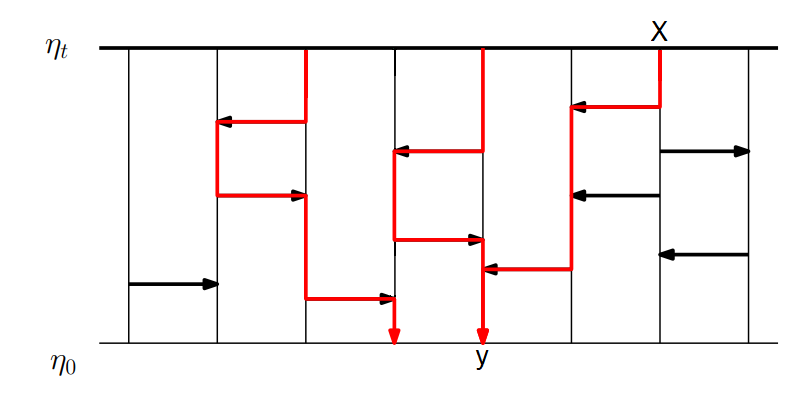
\includegraphics[width=0.7\textwidth]{immagini/harris}\caption{\label{fig:Harris}Example of Harris\textquoteright{} graphical construction
of the voter model on a one dimensional lattice (from \cite{schertzer_brownian_2017}) }

\end{figure}

To identify $\eta_{t}\left(x\right)$, we just need to work down the
graphical representation, i.e. trace the \textit{genealogy} of where
the opinion $\eta_{t}\left(x\right)$ comes from backward in time.
For example, in fig \ref{fig:Harris} to obtain the opinion at $t$
in $x$, we need to follow the arrows backward in time, until we reach
the origin $y$ of the walk at time $0$. It should be clear that
$\eta_{t}\left(x\right)=\eta_{0}\left(y\right)$. The genealogy line
$\pi_{t}^{x,t}$ for $\eta_{t}\left(x\right)$ is then a continuous
time random walk running backward in time that jumps at rate $1$.
In wider terms, we have:
\begin{equation}
\eta_{t}\left(x\right)=n_{t-s}\left(\pi_{s}^{x,t}\right).\label{eq:dual}
\end{equation}
Moreover, by construction we can observe that if two genealogy lines
collide at time $s$, i.e. $\pi_{s}^{x,t}=\pi_{s}^{x',t}$ for some
$s$, then the two random walks will stay together at \textit{earlier}
times. For these reasons we say that the voter model and the \textit{coalescing
random walks} are dual to one another. In other terms, we can say
that:
\begin{equation}
\mathbb{P}\left(\eta_{t}\left(x\right)=1\quad\forall x\in B\right)\text{=}\mathbb{P}\left(\eta_{0}\left(y\right)=1\quad\forall y\in\pi_{t}^{B}\right)\label{eq:dual_P}
\end{equation}
where $\pi_{t}^{B}$ is a set-valued dual process starting from each
point of $B$. 

Now we can formulate the Holley and Liggett's theorem \cite{LiggettH1975}:
\begin{thm}
\label{thm:voter}In $d\leq2$ the voter model approaches complete
consensus, i.e. as $t\to\infty$ $\mathbb{P}\left(\eta_{t}\left(x\right)=\eta_{t}\left(y\right)\right)=1$.
In $d\geq3$ if we assign opinions $1$ and $0$ independently to
sites with probabilities $u$ and $1-u$ then as $t\rightarrow+\infty$,
$\eta_{t}^{u}$ converges in distribution to $\eta_{+\infty}^{u}$,
a stationary distribution, $\nu_{u}$, in which a fraction $u$ of
the sites have opinion $1$. 
\end{thm}


\section{The voter model perturbations\label{sec:Voter-model-perturbation}}

Now, we want to analyse the connection between the interacting particle
system and the dynamical systems. Cox, Durrett and Perkins in \cite{cox_voter_2011}
rigorously showed this connection and formulated a reaction-diffusion
equation for the small perturbed voter model. 

In \cite{durrett_spatial_2014,cox_voter_2011} they studied a class
of interacting particle systems on $\mathbb{Z}^{d}$ whose transition
rate is a small perturbation of the transition rate of a voter model.
We choose the Birth-Death dynamics, so that the transition rate is:
\begin{equation}
c\left(x,\eta\right)=\sum_{y}p\left(y-x\right)\left[\mathbf{1}_{\left\{ \eta\left(y\right)\neq\eta\left(x\right)\right\} }+\varepsilon^{2}A_{\eta\left(x\right),\eta\left(y\right)}\right]\label{eq:perturbation}
\end{equation}

where the perturbation parameter is $0<\epsilon\ll1$ and, considering
the opinion $\eta\left(x\right)$ as the strategy of the voter in
$x$, $A_{\eta\left(x\right),\eta\left(y\right)}$ is the payoff of
the player in $x$ playing $\eta\left(x\right)$ against the player
in $y$ playing $\eta\left(y\right)$ in the game with the payoff
matrix \ref{eq:payoff}. In other words, we can see the transition
rate $c\left(x,\eta\right)$ as the payoff of the voter in $x$ playing
the strategy $\eta\left(x\right)$ against all the neighbouring voters
in $y$ playing $\eta\left(y\right)$. It can be shown that the perturbation
term is:
\begin{equation}
h_{i,j}\left(0,\eta\right)=\sum_{k}\sum_{x}\sum_{y}p\left(y-x\right)p\left(x\right)\mathbf{1}_{\left\{ \eta\left(x\right)=j,\eta\left(y\right)=k\right\} }A_{j,k}\label{eq:hij}
\end{equation}

In \cite{cox_voter_2011,durrett_spatial_2014} the following theorem
is enunciated and proved.
\begin{thm}
\label{thm:RDE-ips}Suppose $d\geq3$. Let $v_{i}\,:\,\mathbb{R}^{d}\rightarrow\left[0,1\right]$
be continuous with $\sum_{i\in\mathbb{Z}^{d}}v_{i}=1$. Let $\eta_{0}^{\varepsilon}$
be the initial conditions of the process with perturbed flip rates
with local density $v_{i}$ and let: 
\[
u_{i}^{\varepsilon}\left(x,t\right)=\mathbb{P}\left(\eta_{t\varepsilon^{-2}}^{\varepsilon}\left(x\right)=i\right)
\]
 If $x_{\varepsilon}\rightarrow x$ as $\varepsilon\to0$ then $u_{i}^{\varepsilon}\left(x_{\varepsilon},t\right)$
converges to $u_{i}\left(x,t\right)$, the solution of the following
system of partial differential equations: 
\begin{equation}
\frac{\partial u_{i}\left(x,t\right)}{\partial t}=\frac{\sigma^{2}}{2}\Delta u_{i}\left(x,t\right)+\phi_{i}\left(u\left(x,t\right)\right)\label{eq:rde}
\end{equation}
with initial condition $u_{i}\left(x,0\right)=v_{i}\left(x\right)$
and $\frac{\sigma^{2}}{2}$ depends on the topology of the lattice.
The reaction term: 
\begin{equation}
\phi_{i}\left(u\right)=\sum_{j\neq i}\left\langle \mathbf{1}_{\left\{ \eta\left(0\right)=j\right\} }h_{j,i}\left(0,\eta\right)-\mathbf{1}_{\left\{ \eta\left(0\right)=i\right\} }h_{i,j}\left(0,\eta\right)\right\rangle _{u}\label{eq:reactionterm}
\end{equation}
where $\left\langle \cdot\right\rangle $ is the expected value with
respect to the voter model stationary distribution $v_{u}$ in which
the densities are given by the vector $u$.
\end{thm}

Intuitively, the process is always close to the voter equilibrium
for the current density vector $u$, when on the time scale the voter
model runs at rate $\varepsilon^{-2}$ versus the perturbation at
rate $1$. Thus, the rate of change of $u_{i}$ depends on the nearby
sites assumed to be in that voter model equilibrium. We restrict to
dimensions $d\geq3$ because, as seen in theorem \ref{thm:voter},
the voter model does not have nontrivial stationary distributions
in $d\leq2$.

\section{The modified game}

Now, we can compute $\phi_{i}\left(u\right)$ for the Birth-Death
dynamics. Inserting the term \ref{eq:hij} in \ref{eq:reactionterm}
we obtain:
\begin{align*}
\phi_{i}\left(u\right) & =\left\langle \sum_{j\neq i}\mathbf{1}_{\left\{ \eta\left(0\right)=j\right\} }\sum_{k}\sum_{x}\sum_{y}p\left(y-x\right)p\left(x\right)\mathbf{1}_{\left\{ \eta\left(x\right)=i,\eta\left(y\right)=k\right\} }A_{i,k}\right.\\
 & -\left.\sum_{j\neq i}\mathbf{1}_{\left\{ \eta\left(0\right)=i\right\} }\sum_{k}\sum_{x}\sum_{y}p\left(y-x\right)p\left(x\right)\mathbf{1}_{\left\{ \eta\left(x\right)=j,\eta\left(y\right)=k\right\} }A_{j,k}\right\rangle \\
 & =\sum_{j\neq i}\sum_{k}q\left(j,i,k\right)A_{i,k}-q\left(i,j,k\right)A_{j,k}
\end{align*}
where the quantity: 
\[
q\left(i,j,k\right)=\mathbb{P}\left(\eta\left(0\right)=i,\eta\left(v_{1}\right)=j,\eta\left(v_{1}+v_{2}\right)=k\right)
\]
and $v_{1}$and $v_{2}$ are independent and chosen according to the
distribution $p$. We have for $i\neq j$:
\begin{align*}
q\left(i,j,k\right) & =p\left(0\mid v_{1}\mid v_{1}+v_{2}\right)u_{i}u_{j}u_{k}\\
 & +\mathbf{\mathbf{1}}_{\left\{ i=k\right\} }p\left(0,v_{1}+v_{2}\mid v_{1}\right)u_{i}u_{j}\\
 & +\mathbf{\mathbf{1}}_{\left\{ j=k\right\} }p\left(0\mid v_{1},v_{1}+v_{2}\right)u_{i}u_{j}
\end{align*}
 Here, we use Durret's notation where:
\begin{itemize}
\item $p\left(x\mid y\mid z\right)$ is the probability that the three random
walks never hit;
\item $p\left(x\mid y,z\right)$ is the probability that the walks starting
from $y$ and $z$ coalesce, but they do not hit the one starting
at $x$. 
\end{itemize}
So, inserting $q\left(i,j,k\right)$ in $\phi_{i}\left(u\right)$
, we have:
\begin{align*}
\phi_{i}\left(u\right) & =p\left(0\mid v_{1}\mid v_{1}+v_{2}\right)\sum_{j\neq i}\sum_{k}u_{i}u_{j}u_{k}\left(A_{i,k}-A_{j,k}\right)\\
 & +p\left(0,v_{1}+v_{2}\mid v_{1}\right)\sum_{j\neq i}u_{i}u_{j}\left(A_{i,j}-A_{j,i}\right)\\
 & +p\left(0\mid v_{1},v_{1}+v_{2}\right)\sum_{j\neq i}u_{i}u_{j}\left(A_{i,i}-A_{j,j}\right)
\end{align*}
It can be shown that:
\[
p\left(0,v_{1}+v_{2}\mid v_{1}\right)=p\left(0\mid v_{1},v_{1}+v_{2}\right)
\]
 and we have:
\begin{align*}
\phi_{i}\left(u\right) & =p\left(0\mid v_{1}\mid v_{1}+v_{2}\right)\sum_{j\neq i}\sum_{k}u_{i}u_{j}u_{k}\left(A_{i,k}-A_{j,k}\right)\\
 & +p\left(0\mid v_{1},v_{1}+v_{2}\right)\sum_{j\neq i}u_{i}u_{j}\left(A_{i,j}-A_{j,i}+A_{i,i}-A_{j,j}\right)
\end{align*}
The first term in the RHS is the replicator equation:
\[
\frac{du_{i}}{dt}=\sum_{j\neq i}\sum_{k}u_{i}u_{j}u_{k}\left(A_{i,k}-A_{j,k}\right)=\phi_{R}^{i}\left(u\right)
\]
If coalescing is impossible $p\left(0\mid v_{1}\mid v_{1}+v_{2}\right)=1$
and $p\left(0\mid v_{1},v_{1}+v_{2}\right)=0$, then $\phi_{i}=\phi_{R}^{i}$.
Now, let:
\[
M_{i,j}=\frac{p\left(0\mid v_{1},v_{1}+v_{2}\right)}{p\left(0\mid v_{1}\mid v_{1}+v_{2}\right)}\left(A_{i,j}-A_{j,i}+A_{i,i}-A_{j,j}\right)
\]
This matrix is skew symmetric $M_{i,j}=-M_{j,i}$ so $\sum_{i,j}u_{i}M_{i,j}u_{j}=0$
and we obtain:
\begin{align*}
\phi_{i}\left(u\right) & =p\left(0\mid v_{1}\mid v_{1}+v_{2}\right)\sum_{j\neq i}\sum_{k}u_{i}u_{j}u_{k}\left(A_{i,k}-A_{j,k}\right)\\
 & +p\left(0\mid v_{1}\mid v_{1}+v_{2}\right)\sum_{j\neq i}u_{i}u_{j}M_{i,j}
\end{align*}
We can easily prove that $\phi_{i}\left(u\right)$ is $p\left(0\mid v_{1}\mid v_{1}+v_{2}\right)$
times the RHS of the replicator equation for the modified game with
a payoff matrix $A+M$.

Moreover, it can be shown that:
\begin{align*}
p\left(0\mid v_{1}\right) & =2p\left(0\mid v_{1},v_{1}+v_{2}\right)+p\left(0\mid v_{1}\mid v_{1}+v_{2}\right)\\
p\left(0\mid v_{1}\right) & =\frac{1}{\kappa-1}
\end{align*}
where $\kappa$ is the number of neighbours of each site on the lattice.
Under the pair approximation, the coalescence of $0$ and $v_{1}$
is assumed independent of the coalescence of $v_{1}$ and $v_{1}+v_{2}$\cite{durrett_spatial_2014},
so: 
\[
\frac{p\left(0\mid v_{1},v_{1}+v_{2}\right)}{p\left(0\mid v_{1}\mid v_{1}+v_{2}\right)}=\frac{p\left(v_{1},v_{1}+v_{2}\right)}{p\left(v_{1}\mid v_{1}+v_{2}\right)}=\frac{1}{\kappa-2}
\]
Finally, the complete equation is:
\begin{align}
\frac{\partial u_{i}\left(x,t\right)}{\partial t} & =\frac{1}{\kappa}\Delta u_{i}\left(x,t\right)+p\left(0\mid v_{1}\mid v_{1}+v_{2}\right)\phi_{i}\left(u\right)\label{eq:RDE_durr}
\end{align}
where $\phi_{i}\left(u\right)$ is the replicator equation for the
modified game with a payoff matrix: 
\begin{equation}
A+M=\left\{ A_{i,j}+\frac{1}{\kappa-2}\left(A_{i,j}-A_{j,i}+A_{i,i}-A_{j,j}\right)\right\} \label{eq:A+M}
\end{equation}
 and by similar observation done in section \ref{sec:A-heuristic-derivation},
we assume $\frac{\sigma^{2}}{2}=\frac{1}{\kappa}$. Now the problem
is to evaluate the quantity $p\left(0\mid v_{1}\mid v_{1}+v_{2}\right)$.
The only way to do it is numerically, but this is beyond the scope
of this paper. The works of Durrett and Yuan Zhang suggest that $p\left(0\mid v_{1}\mid v_{1}+v_{2}\right)\in\left[0.32,\ 0.33\right]$.

Then, we can use this model for the prisoner's dilemma. Recalling
the payoff matrix: 
\[
A=\left(\begin{array}{cc}
1 & 0\\
b & 0
\end{array}\right)
\]
 the matrix $M$ has the following form:
\begin{align*}
M & =\left(\begin{array}{cc}
0 & \frac{1}{\kappa-2}\left(1-b\right)\\
-\frac{1}{\kappa-2}\left(1-b\right) & 0
\end{array}\right)
\end{align*}
 and so the modified payoff matrix is:
\[
A+M=\left(\begin{array}{cc}
1 & \frac{1}{\kappa-2}\left(1-b\right)\\
b-\frac{1}{\kappa-2}\left(1-b\right) & 0
\end{array}\right)
\]


\section{The simulations\label{sec:The-simulations-2}}

Now, we solve the equation \ref{eq:RDE_durr} for the prisoner's dilemma.
It is a parabolic partial differential equation, so we use the Crank-Nicolson,
seen in section \ref{sec:Parabolic-dynamic}. As done for the previous
models, we will study the dynamics \ref{eq:RDE_durr} on a two dimensional
plane $\left[0,L_{x}\right]\times\left[0,L_{y}\right]$ in a time
interval $\left[0,T\right]$. The equation is endowed with the initial
conditions:
\begin{align*}
u_{1}\left(x,y,0\right) & =u_{1}^{0}\left(x,y\right)\\
u_{2}\left(x,y,0\right) & =u_{2}^{0}\left(x,y\right)
\end{align*}
and we choose three forms of $u_{1}^{0}\left(x,y\right)$ and $u_{2}^{0}\left(x,y\right)$:
\begin{enumerate}
\item a random value between $0$ to $1$ for $u_{1}^{0}$ and $u_{2}^{0}=1-u_{1}^{0}$,
i.e.: 
\begin{align*}
\forall x,y\quad u_{1}^{0}\left(x,y\right) & =random\left[0,1\right]\\
\forall x,y\quad u_{2}^{0}\left(x,y\right) & =1-u_{1}^{0}\left(x,y\right)
\end{align*}
\item the population of the defectors is concentrated in a single point
in a sea of cooperators, i.e. for the cooperators:
\[
u_{1}^{0}\left(x,y\right)=\begin{cases}
1 & if\ x\neq\frac{L_{x}}{2}\ or\ y\neq\frac{L_{y}}{2}\\
0 & otherwise
\end{cases}
\]
 and for the defectors:
\[
u_{2}^{0}\left(x,y\right)=\begin{cases}
1 & if\ x=\frac{L_{x}}{2}\ and\ y=\frac{L_{y}}{2}\\
0 & otherwise
\end{cases};
\]
\item the portion of the defector agents is arranged as a delta distribution
surrounded by cooperators, i.e.:
\begin{align*}
u_{1}^{0}\left(x,y\right) & =\begin{cases}
1 & if\ x\neq\frac{L_{x}}{2}\\
0 & otherwise
\end{cases}\\
u_{2}^{0}\left(x,y\right) & =\begin{cases}
1 & if\ x=\frac{L_{x}}{2}\\
0 & otherwise
\end{cases}
\end{align*}
\end{enumerate}
And the chosen boundary conditions are zero, i.e. for $i=1,2$:
\[
u_{i}\left(0,0,t\right)=u_{i}\left(0,L_{y},t\right)=u_{i}\left(L_{x},0,t\right)=u_{i}\left(L_{x},L_{y},t\right)=0\quad\forall t\in\left[0,T\right].
\]


\subsection{Random initial condition}

First, we study the evolution of \ref{eq:RDE_durr} with a random
initial position of cooperators and defectors (fig \ref{fig:rand-2}). 

\begin{figure}
\subfloat[]{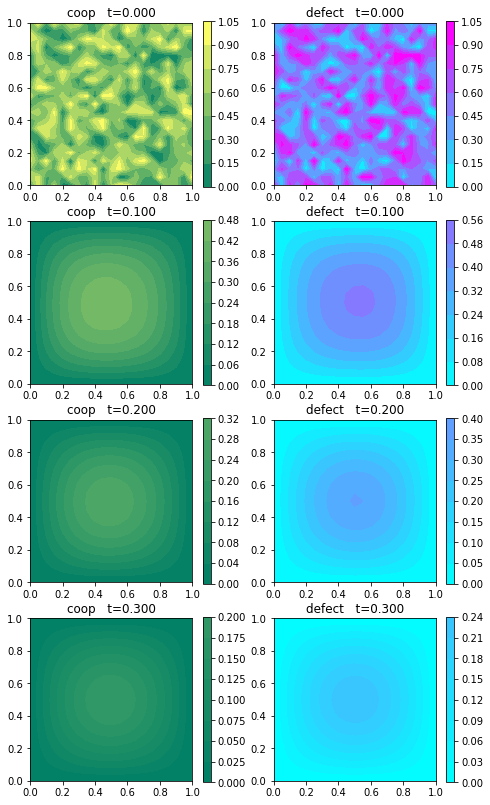
\includegraphics[width=0.5\textwidth]{immagini/durr-rand4}

}\subfloat[]{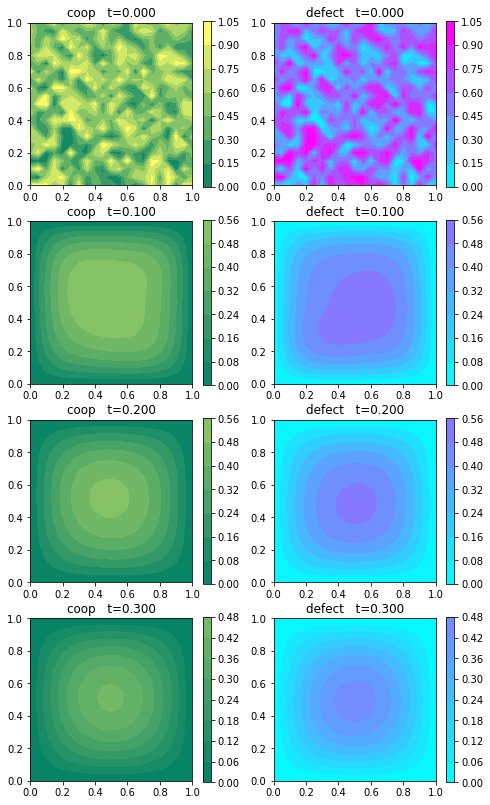
\includegraphics[width=0.5\textwidth]{immagini/durr-rand8}

}\caption{\label{fig:rand-2}Numerical solution of $u_{1}$ and $u_{2}$ in
$T=0.3$ and $L_{x}=L_{y}=20$ of \ref{eq:RDE_durr} using Crank-Nicolson
with $\kappa=4$ (A) and $\kappa=8$ (B). For both the methods we
set $N_{x}=N_{y}=20$, $dt=0.001$ and $b=1.85$.}
\end{figure}


\subsection{One defector in a sea of cooperators}

Secondly, we study the two equations setting at the starting time
the defectors in a single central point (fig \ref{fig:onedef-2}). 

\begin{figure}
\subfloat[]{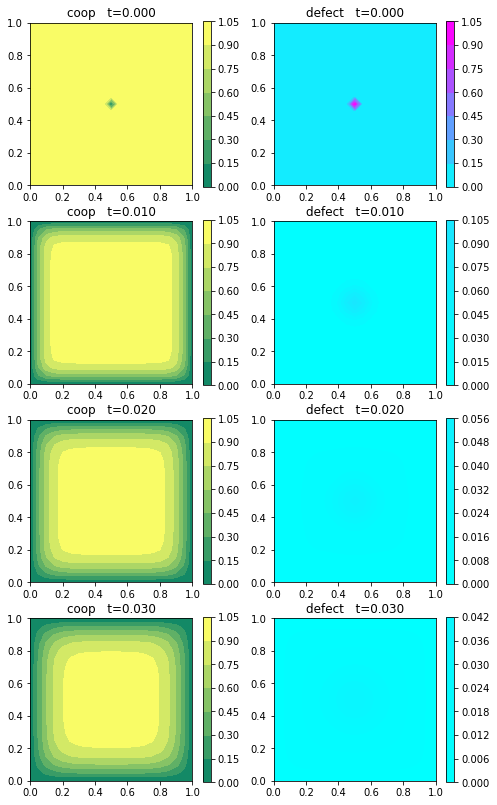
\includegraphics[width=0.5\textwidth]{immagini/durr-onedef4}

}\subfloat[]{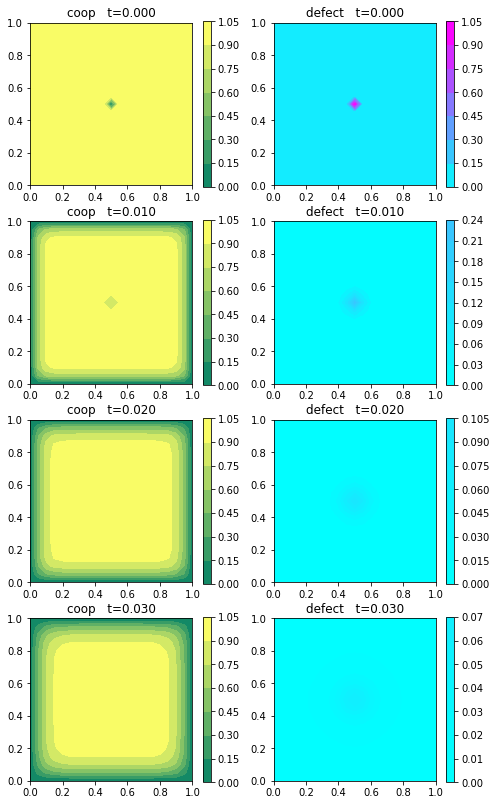
\includegraphics[width=0.5\textwidth]{immagini/durr-onedef8}

}

\caption{\label{fig:onedef-2}Numerical solution of $u_{1}$ and $u_{2}$ in
$T=0.3$ and $L_{x}=L_{y}=20$ of \ref{eq:RDE_durr} using Crank-Nicolson
with $\kappa=4$ (A) and $\kappa=8$ (B). For both the methods we
set $N_{x}=N_{y}=20$, $dt=0.001$ and $b=1.85$.}
\end{figure}


\subsection{Delta initial condition}

Finally, we analyse the two models, arranging the defectors in delta-type
function in the space surrounded by the cooperators, at the initial
time (fig \ref{fig:delta-2}). 

\begin{figure}
\subfloat[]{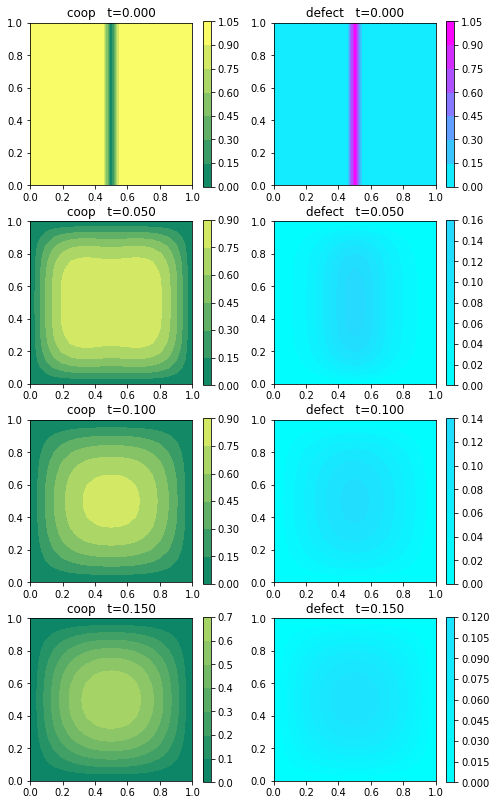
\includegraphics[width=0.5\textwidth]{immagini/durr-delta4}

}\subfloat[]{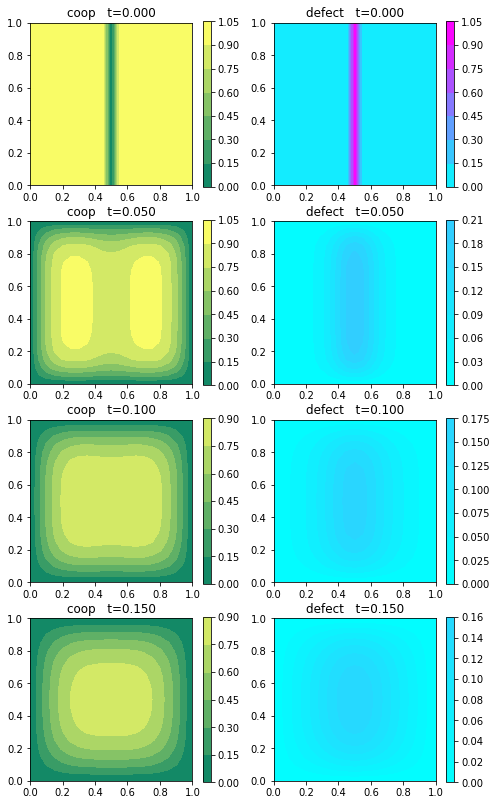
\includegraphics[width=0.5\textwidth]{immagini/durr-delta8}

}

\caption{\label{fig:delta-2}Numerical solution of $u_{1}$ and $u_{2}$ in
$T=0.3$ and $L_{x}=L_{y}=20$ of \ref{eq:RDE_durr} using Crank-Nicolson
with $\kappa=4$ (A) and $\kappa=8$ (B). For both the methods we
set $N_{x}=N_{y}=20$, $dt=0.001$ and $b=1.85$.}
\end{figure}


\subsection{Phase diagram and conclusions}

Here, it seems that the evolution is quite different from the previous
models, and in the last two cases the defectors do not invade the
whole of the space. But this is a fallacy, because we are considering
too short time frame predictions. Indeed, varying the value of $b$
and letting the evolution runs for $t\rightarrow+\infty$ (in practice
for $t$ sufficiently long) we can plot the phase diagrams of the
probability of a strategy.

\begin{figure}
\subfloat[]{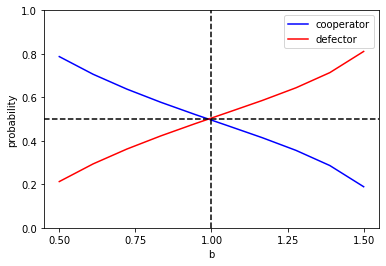
\includegraphics[width=0.5\textwidth]{immagini/durr4_phase}}\subfloat[]{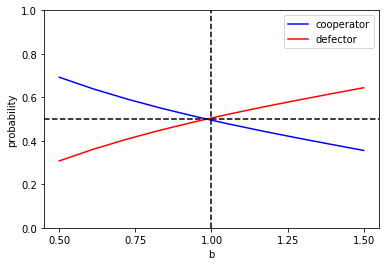
\includegraphics[width=0.5\textwidth]{immagini/durr8_phase}}\caption{Phase diagrams of the \ref{eq:RDE_durr} with 4 nearest neighbour
(A) and with 8 nearest neighbour (B).}
\end{figure}
Not so surprisingly, we observe a phase transition when $b=1$. Recalling
the payoff matrix:
\[
A=\left(\begin{array}{cc}
R & S\\
T & P
\end{array}\right)=\left(\begin{array}{cc}
1 & 0\\
b & 0
\end{array}\right)
\]
 we have a phase transition when the payoff of the defection (i.e.
the temptation $T$) becomes higher than the one for the cooperation
(i.e. the reward $R$). 



\part*{Conclusions}
\noindent \begin{flushright}
\textit{Not only in research, but also in the everyday world}\\
\textit{ of politics and economics, we would all be better off}\\
\textit{ if more people realised that simple nonlinear systems}\\
\textit{ do not necessarily possess simple dynamical properties.}\\
Robert May
\par\end{flushright}

We studied the evolution of different populations that are in the
same environment, using evolutionary game theory. We investigated
the prisoner's dilemma, where the population is composed by the cooperators
which are friendly and the defectors which are hostile. The payoff
matrix for our game is:
\[
\left(\begin{array}{cc}
1 & 0\\
b & 0
\end{array}\right)
\]
Our main interest was about the survival of cooperators, which is
impossible in classical game theory (i.e. in in the spatially homogeneous
case) as observed in Nowak's works (e.g. \cite{nowak_evolutionary_1992,nowak_more_1994,nowak_spatial_1993,nowak_spatial_1994}).
So, in this work we studied and compared four models of evolutionary
games that consider spatial effects. 
\begin{enumerate}
\item The first model is a reaction diffusion equation, proposed by Vickers
\cite{vickers_spatial_1989}, for $\ell=1,\,2$:
\[
\frac{\partial n_{\ell}}{\partial t}=n_{\ell}\left[\frac{\mathbf{e}_{\ell}^{T}A\,\mathbf{n}}{N}-\frac{\mathbf{n}^{T}A\,\mathbf{n}}{N^{2}}\right]+D_{\ell}\nabla^{2}n_{\ell}
\]
where the reaction term is the replicator dynamic and $D_{\ell}$is
an arbitrary constant. The central assumption of diffusive movement
involves that the individuals move with infinite velocity. This does
not mean that diffusion models are completely inappropriate rather,
it only means that these models are more accurate in long time frame
predictions. For example several diffusion models are used for distributions
of insects in the atmosphere, for homing and migration of birds and
fishes, or even for some mammals migration (for more details \cite{murray1,murray2,Okubo_Levin}).
In our simulations we merely observe that there is no survival of
cooperators, i.e. the evolutionarily stable strategy does not change
considering spatial effect. Moreover, as verification through the
phase diagram we simply observe a phase transition in $b=1$.
\item The second model, in practice, is a correction to the first model.
It is a continuous finite propagation speed model for population dynamics,
based on a hyperbolic Cattaneo dynamics for the flux function. This
model is a midway between the multi agent system and the continuous
reaction-diffusion models, i.e. for $\ell=1,\,2$:
\[
\begin{cases}
\frac{\partial n_{\ell}}{\partial t} & =-\left(\frac{\partial\varphi_{\ell}}{\partial x}+\frac{\partial\psi_{\ell}}{\partial y}\right)+n_{\ell}\left[\frac{\mathbf{e_{\ell}}^{T}A\,\mathbf{n}}{N}-\frac{\mathbf{n}^{T}A\,\mathbf{n}}{N^{2}}\right]\\
\tau\frac{\partial\varphi_{\ell}}{\partial t} & =-\lambda_{\ell}^{2}\frac{\partial n_{\ell}}{\partial x}-\varphi_{\ell}\\
\tau\frac{\partial\psi_{\ell}}{\partial t} & =-\lambda_{\ell}^{2}\frac{\partial n_{\ell}}{\partial y}-\psi_{\ell}
\end{cases}
\]
where $\tau$ is the relaxation time, $\lambda_{\ell}$ is related
to the dispersal rate, $\varphi_{\ell}$ is the flux along $x$ and
$\psi_{\ell}$ the one along $y$. In our simulations there is no
survival of cooperators. So requiring a finite speed of diffusion
is not enough to have the same results of Nowak's models.
\item In the second chapter, we proposed a discrete model. We assume that
the agents move randomly on a square 2D lattice under the effect of
a drift term due to the discrete replicator equation, for $\ell=1,\,2$:
\begin{align*}
n_{\ell}^{k+1}(x) & =\frac{1}{2m}\sum_{y\in U(x)}\mathcal{L}_{xy}n_{\ell}^{k}\left(y\right)+n_{\ell}^{k}\left(x\right)\frac{c+\frac{{\bf e}_{\ell}\cdot A{\bf n}^{k}\left(x\right)}{N^{k}\left(x\right)}}{c+\frac{{\bf n}^{k}\left(x\right)\cdot A{\bf n}^{k}\left(x\right)}{\left(N^{k}\left(x\right)\right)^{2}}}
\end{align*}
The results are similar to the previous models, but now the number
of cooperators and defectors decreases at a slower speed. This is
an interesting results, because we made no hypothesis and no requirement
on the dispersal speed. 
\item In the last model we considered the games as a a perturbed voter model.
In \cite{durrett_spatial_2014,cox_voter_2011}, they showed that the
evolution of these games convergences to solutions of a reaction diffusion
equation (RDE), for $i=1,\,2$:
\[
\frac{\partial u_{i}\left(x,t\right)}{\partial t}=\frac{1}{\kappa}\Delta u_{i}\left(x,t\right)+p\left(0\mid v_{1}\mid v_{1}+v_{2}\right)\phi_{i}\left(u\right)
\]
where $\kappa$ is the number of neighbours and $\phi_{i}\left(u\right)$
is the replicator equation for the modified game with a payoff matrix:
\[
\left(\begin{array}{cc}
1 & \frac{1}{\kappa-2}\left(1-b\right)\\
b-\frac{1}{\kappa-2}\left(1-b\right) & 0
\end{array}\right)
\]
We simulate the equation in $2D$ and, as we expect, we observe a
complete consensus, or rather we observe no coexistence of cooperators
and defectors.
\end{enumerate}




\part*{Appendix}
\noindent \begin{flushright}
\textit{The whole history of physics proves}\\
\textit{ that a new discovery is quite likely}\\
\textit{ lurking at the next decimal place.}\\
Floyd Karker Richtmyer
\par\end{flushright}

\section*{Implementation of Crank-Nicolson }

Thanks to the good lectures of Hans Petter Langtangen \cite{langtangen_finite_nodate}
we implemented Crank-Nicolson through the $\theta-rule$ in Python
3 for the parabolic model \ref{eq:vick}. The $\theta-rule$ allows
us to pass from Crank-Nicolson to Forward or Backwark Euler, just
changing the value of a constant $\theta$. 

\begin{lstlisting}
import scipy.sparse
import scipy.sparse.linalg
import numpy as np
import matplotlib.pyplot as plt

def theta2D(
    Ic, Id, a, b, Lx, Ly, Nx, Ny, dt, T, theta=0.5,
    n_0x=0, n_0y=0, n_Lx=0, n_Ly=0,rand=False,plot='OFF',plotN='OFF'):
    
    x = np.linspace(0, Lx, Nx+1)       # mesh points in x dir
    y = np.linspace(0, Ly, Ny+1)       # mesh points in y dir
    dx = x[1] - x[0]                   # distance of mesh points in x dir 
    dy = y[1] - y[0]                   # distance of mesh points in y dir 

    dt = float(dt)   				  # time step
    Nt = int(round(T/float(dt)))       #number of mesh points in time
    t = np.linspace(0, Nt*dt, Nt+1)    # mesh points in time

    #CFL numbers
    Fx = a*dt/dx**2
    Fy = a*dt/dy**2
    
    #plot a graph 3 times, i.e. 1st plot at t=Nim, 
	#2nd plot at t=2*Nim, 3rd plot at t=3*Nim
    Nim= int(Nt/3)
    im=0 #index for subplot
    
    #Payoff matrix
    a11=1.0
    a12=0
    a21=b
    a22=0   
        
    n1  = np.zeros((Nx+1, Ny+1))    # unknown n1 at new time level
    n1_ = np.zeros((Nx+1, Ny+1))    # n1 at the previous time level
    n2  = np.zeros((Nx+1, Ny+1))    # unknown n2 at new time level
    n2_ = np.zeros((Nx+1, Ny+1))    # n2 at the previous time level
    
    #useful vectors to call a mesh point in each direction
    Ix = range(0, Nx+1)
    Iy = range(0, Ny+1)
    It = range(0, Nt+1)

    # Make n_0x, n_0y, n_Lx and n_Ly functions if they are float/int
    if isinstance(n_0x, (float,int)):
        _n_0x = float(n_0x)  # Make copy of n_0x
        n_0x = lambda t: _n_0x
    if isinstance(n_0y, (float,int)):
        _n_0y = float(n_0y)  # Make copy of n_0y
        n_0y = lambda t: _n_0y
    if isinstance(n_Lx, (float,int)):
        _n_Lx = float(n_Lx)  # Make copy of n_Lx
        n_Lx = lambda t: _n_Lx
    if isinstance(n_Ly, (float,int)):
        _n_Ly = float(n_Ly)  # Make copy of n_Ly
        n_Ly = lambda t: _n_Ly

    # Load initial conditions into n1_ and n2_
    #random initial conditions
    if rand==True:
        n_r=np.random.rand(Nx+1, Ny+1)
        n1_ = n_r
        n2_ = 1-n_r
    #other initial conditions
    else:
        for i in Ix:
            for j in Iy:
                n1_[i,j] = Ic(i,j)
                n2_[i,j] = Id(i,j)
        
    
    #set size and features of the plot of the total population
    if plotN=='ON':
        fig1 = plt.figure(figsize=(5,5))           
        ax1 = fig1.add_subplot(1,1,1)
        ax1.set_title('Number of total players (N)')
        ax1.set_xlabel('time (n*dt)')
        ax1.set_ylabel('N')
    
    #plot the initial conditions
    if plot=='ON':
        fig = plt.figure(figsize=(8,14))
        im+=1
        ax = fig.add_subplot(4,2,im)
        ax.set_aspect('equal')
        cc1=plt.contourf(x, y, n1_,cmap="summer",vmin=0, vmax=1)
        fig.colorbar(cc1)
        ax.set_title('coop   t=%1.3f' %(0))

        im+=1
        ax = fig.add_subplot(4,2,im)
        ax.set_aspect('equal')
        cc2=plt.contourf(x, y, n2_,cmap="cool",vmin=0, vmax=1)
        fig.colorbar(cc2)
        ax.set_title('defect   t=%1.3f' %(0))
        


    
    # Two-dim coordinate arrays for vectorized function evaluations
    xv = x[:,np.newaxis]
    yv = y[np.newaxis,:]

    
    N = (Nx+1)*(Ny+1)
    #Allocate the matrix A1
    mainc   = np.zeros(N)            # diagonal
    lowerc  = np.zeros(N-1)          # subdiagonal
    upperc  = np.zeros(N-1)          # superdiagonal
    lower2c = np.zeros(N-(Nx+1))     # lower diagonal
    upper2c = np.zeros(N-(Nx+1))     # upper diagonal
    #Allocate c1, i.e. the RHS
    c1      = np.zeros(N)
    
    #Allocate the matrix A2
    maind   = np.zeros(N)            # diagonal
    lowerd  = np.zeros(N-1)          # subdiagonal
    upperd  = np.zeros(N-1)          # superdiagonal
    lower2d = np.zeros(N-(Nx+1))     # lower diagonal
    upper2d = np.zeros(N-(Nx+1))     # upper diagonal
    #Allocate c2, i.e. the RHS
    c2      = np.zeros(N)

    # Precompute sparse matrix
    lower_offsetc = 1
    lower2_offsetc = Nx+1
    
    lower_offsetd = 1
    lower2_offsetd = Nx+1

    #mapping function of the mesh points
    m = lambda i, j: j*(Nx+1) + i
    
    #Build the matrices A1 and A2
    # j=0 boundary line
    j = 0; mainc[m(0,j):m(Nx+1,j)] = 1  
    j = 0; maind[m(0,j):m(Nx+1,j)] = 1
    
    
    for j in Iy[1:-1]:             # Interior mesh lines j=1,...,Ny-1
        i = 0;   mainc[m(i,j)] = 1  # Boundary
        i = Nx;  mainc[m(i,j)] = 1  # Boundary
        
        i = 0;   maind[m(i,j)] = 1  # Boundary
        i = Nx;  maind[m(i,j)] = 1  # Boundary
        
        
        # Interior i points: i=1,...,N_x-1
        lower2c[m(1,j)-lower2_offsetc:m(Nx,j)-lower2_offsetc] = - theta*Fy
        lowerc[m(1,j)-lower_offsetc:m(Nx,j)-lower_offsetc] = - theta*Fx
        mainc[m(1,j):m(Nx,j)] = 1 + 2*theta*(Fx+Fy)
        upperc[m(1,j):m(Nx,j)] = - theta*Fx
        upper2c[m(1,j):m(Nx,j)] = - theta*Fy
        
        lower2d[m(1,j)-lower2_offsetd:m(Nx,j)-lower2_offsetd] = - theta*Fy
        lowerd[m(1,j)-lower_offsetd:m(Nx,j)-lower_offsetd] = - theta*Fx
        maind[m(1,j):m(Nx,j)] = 1 + 2*theta*(Fx+Fy)
        upperd[m(1,j):m(Nx,j)] = - theta*Fx
        upper2d[m(1,j):m(Nx,j)] = - theta*Fy
    
    
    j = Ny; mainc[m(0,j):m(Nx+1,j)] = 1  # Boundary line
    j = Ny; maind[m(0,j):m(Nx+1,j)] = 1  # Boundary line
    
    #Built the matrices as sparse matrices
    A1 = scipy.sparse.diags(
        diagonals=[mainc, lowerc, upperc, lower2c, upper2c],
        offsets=[0, -lower_offsetc, lower_offsetc,
                 -lower2_offsetc, lower2_offsetc],
        shape=(N, N), format='csc')
    
    A2 = scipy.sparse.diags(
        diagonals=[maind, lowerd, upperd, lower2d, upper2d],
        offsets=[0, -lower_offsetc, lower_offsetc,
                 -lower2_offsetd, lower2_offsetd],
        shape=(N, N), format='csc')

    # Evolution start
    for n in It[0:-1]:
        
        # Compute c1 and c2

        j = 0; c1[m(0,j):m(Nx+1,j)] = n_0y(t[n+1])      # Boundary
        j = 0; c2[m(0,j):m(Nx+1,j)] = n_0y(t[n+1])      # Boundary
        for j in Iy[1:-1]:
            i = 0;   p = m(i,j);  c1[p] = n_0x(t[n+1])  # Boundary
            i = Nx;  p = m(i,j);  c1[p] = n_Lx(t[n+1])  # Boundary
            i = 0;   p = m(i,j);  c2[p] = n_0x(t[n+1])  # Boundary
            i = Nx;  p = m(i,j);  c2[p] = n_Lx(t[n+1])  # Boundary
            
            imin = Ix[1]
            imax = Ix[-1]  # for slice, max i index is Ix[-1]-1
            c1[m(imin,j):m(imax,j)] = n1_[imin:imax,j]+ \
                  (1-theta)*(Fx*(n1_[imin+1:imax+1,j]- \
                  2*n1_[imin:imax,j]+n1_[imin-1:imax-1,j])+ \
                  Fy*(n1_[imin:imax,j+1]-2*n1_[imin:imax,j]+ \
                  n1_[imin:imax,j-1]))-dt*((n1_[imin:imax,j]* \
                  n2_[imin:imax,j])/(n1_[imin:imax,j]+ \
                  n2_[imin:imax,j])**2)*((a21-a11)*n1_[imin:imax,j]+ \
                  (a22-a12)*n2_[imin:imax,j])
            
            c2[m(imin,j):m(imax,j)] = n2_[imin:imax,j]+ \
                  (1-theta)*(Fx*(n2_[imin+1:imax+1,j]- \
                  2*n2_[imin:imax,j]+n2_[imin-1:imax-1,j])+ \
                  Fy*(n2_[imin:imax,j+1]-2*n2_[imin:imax,j]+ \
                  n2_[imin:imax,j-1]))+dt*((n1_[imin:imax,j]* \
                  n2_[imin:imax,j])/(n1_[imin:imax,j]+ \
                  n2_[imin:imax,j])**2)*((a21-a11)*n1_[imin:imax,j]+ \
                  (a22-a12)*n2_[imin:imax,j])
            
            
        j = Ny;  c1[m(0,j):m(Nx+1,j)] = n_Ly(t[n+1]) # Boundary
        j = Ny;  c2[m(0,j):m(Nx+1,j)] = n_Ly(t[n+1])

        #Solving the system
        b1 = scipy.sparse.linalg.spsolve(A1, c1)
        b2 = scipy.sparse.linalg.spsolve(A2, c2)
        
        # Fill n1 and n2 with vectors b1 and b2
        #for j in Iy:  # vectorize y lines
        n1[:,:] = b1.reshape(Ny+1,Nx+1).T
        n2[:,:] = b2.reshape(Ny+1,Nx+1).T

        #plot n1 and n2    
        if plot=='ON':
            if (n+1)%Nim==0:
                #fig = plt.figure(figsize=(6,3))
                im+=1
                ax = fig.add_subplot(4,2,im)
                ax.set_aspect('equal')
                cc1=plt.contourf(x, y, n1,cmap="summer",vmin=0, vmax=1)
                fig.colorbar(cc1)
                ax.set_title('coop   t=%1.3f' %((n+1)*dt))

                im+=1
                ax = fig.add_subplot(4,2,im)
                ax.set_aspect('equal')
                cc2=plt.contourf(x, y, n2,cmap="cool",vmin=0, vmax=1)
                fig.colorbar(cc2)
                ax.set_title('defect   t=%1.3f' %((n+1)*dt))
                
        #plot total population n1+n2
        if plotN=='ON':
            ax1.set(ylim=(0, 400))
            N1=ax1.plot(n*dt,np.sum(n1+n2),'r.')    
            
        # Update n1_ and n2_ before next step
        n1_, n1 = n1, n1_
        n2_, n2 = n2, n2_
    
    return n1, n2
\end{lstlisting}


\section*{Implementation of Lax-Wendroff}

We implemented Lax-Wendroff method for the hyperbolic model \ref{eq:2d_nat}
in Python 3. 

\begin{lstlisting}
import numpy as np
from matplotlib import pyplot as plt

def LaxWendroff2D(
			lmb, tau, Ic, Id, b, Lx, Ly, T,
			Nx, Ny, dt,mu,rand=True,plot='ON',plotN='OFF'):
   
    
    x = np.linspace(0, Lx, Nx+1)       # mesh points in x dir
    y = np.linspace(0, Ly, Ny+1)       # mesh points in y dir
    dx = x[1] - x[0]                   # distance of mesh points in x dir 
    dy = y[1] - y[0]                   # distance of mesh points in y dir 

    dt = float(dt)                     # time step
    Nt = int(round(T/float(dt)))       #number of mesh points in time
    t = np.linspace(0, Nt*dt, Nt+1)    # mesh points in time

    
    #plot a graph 3 times, i.e. 1st plot at t=Nim, 
    #2nd plot at t=2*Nim, 3rd plot at t=3*Nim
    Nim= int(Nt/3)
    im=0 #index for subplot
       
    n1_     = np.zeros((Nx+1,Ny+1)) # n1 at the previous time level
    n1      = np.zeros((Nx+1,Ny+1)) # unknown n1 at new time level
    phi1_   = np.zeros((Nx+1,Ny+1)) # phi1 at the previous time level
    phi1    = np.zeros((Nx+1,Ny+1)) # unknown phi1 at new time level
    psi1_   = np.zeros((Nx+1,Ny+1)) # psi1 at the previous time level
    psi1    = np.zeros((Nx+1,Ny+1)) # unknown psi1 at new time level
    n2_     = np.zeros((Nx+1,Ny+1)) # n2 at the previous time level
    n2      = np.zeros((Nx+1,Ny+1)) # unknown n2 at new time level
    phi2_   = np.zeros((Nx+1,Ny+1)) # phi2 at the previous time level
    phi2    = np.zeros((Nx+1,Ny+1)) # unknown phi2 at new time level
    psi2_   = np.zeros((Nx+1,Ny+1)) # psi2 at the previous time level
    psi2    = np.zeros((Nx+1,Ny+1)) # unknown psi2 at new time level

    #payoff matrix
    P=np.array([[1,0],[b,0]])
    
    #artificial viscosity
    Fx=mu
    Fy=mu

    #Load initial conditions
    #random initial conditions
    if rand==True:
        n_r=np.random.rand(Nx+1, Ny+1)
        n1_ = n_r
        n2_ = 1-n_r
        
    #other initial conditions    
    else:
        for i in range(0,Nx+1):
            for j in range(0,Ny+1):
                n1_[i,j] = Ic(i,j)
                n2_[i,j] = Id(i,j)

    #set size and features of the plot of the total population
    if plotN=='ON':
        fig1 = plt.figure(figsize=(5,5))           
        ax1 = fig1.add_subplot(1,1,1)
        ax1.set_title('Number of total players (N)')
        ax1.set_xlabel('time (n*dt)')
        ax1.set_ylabel('N')
    
    #plot the initial conditions
    if plot=='ON':
        fig = plt.figure(figsize=(8,14))
        im+=1
        ax = fig.add_subplot(4,2,im)
        ax.set_aspect('equal')
        cc1=plt.contourf(x, y, n1_,cmap="summer",vmin=0, vmax=1)
        fig.colorbar(cc1)
        ax.set_title('coop   t=%1.3f' %(0))

        im+=1
        ax = fig.add_subplot(4,2,im)
        ax.set_aspect('equal')
        cc2=plt.contourf(x, y, n2_,cmap="cool",vmin=0, vmax=1)
        fig.colorbar(cc2)
        ax.set_title('defect   t=%1.3f' %(0))
    
    # Evolution start        
    for n in range(1,Nt+1):
        for j in range(1,Ny):
            for i in range(1,Nx):
                n1[i,j]  =(n1_[i,j]
                           -dt/(2*dx)*(phi1_[i+1,j]-phi1_[i-1,j])
                           -dt/(2*dy)*(psi1_[i,j+1]-psi1_[i,j-1])
                           +dt**2/(2*dx**2)*(phi1_[i+1,j]
						   -2*phi1_[i,j]+phi1_[i-1,j])
                           +dt**2/(2*dy**2)*(psi1_[i,j+1]
						   -2*psi1_[i,j]+psi1_[i,j-1])
                           +Fx*(n1_[i-1,j] - 2*n1_[i,j] + n1_[i+1,j])
                           +Fy*(n1_[i,j-1] - 2*n1_[i,j] + n1_[i,j+1])
                           -dt*((n1_[i,j]*n2_[i,j])/(n1_[i,j]+n2_[i,j])**2)*
                           ((P[1,0]-P[0,0])*n1_[i,j]
						   +(P[1,1]-P[0,1])*n2_[i,j]))
                
                phi1[i,j]=(phi1_[i,j]
                           -(dt*lmb**2)/(2*dx*tau)*(n1_[i+1,j]-n1_[i-1,j])
                           +((dt*lmb**2)/(2*dx*tau))**2
						   *(n1_[i+1,j]-2*n1_[i,j]+n1_[i-1,j])
                           +Fx*(phi1_[i-1,j] - 2*phi1_[i,j] + phi1_[i+1,j])
                           -dt*phi1_[i,j]/tau)
                
                psi1[i,j]=(psi1_[i,j]
                           -(dt*lmb**2)/(2*dy*tau)*(n1_[i,j+1]-n1_[i,j-1])
                           +((dt*lmb**2)/(2*dy*tau))**2
						   *(n1_[i,j+1]-2*n1_[i,j]+n1_[i,j-1])
                           +Fy*(psi1_[i,j-1] - 2*psi1_[i,j] + psi1_[i,j+1])
                           -dt*psi1_[i,j]/tau)

                n2[i,j]  =(n2_[i,j]
                           -dt/(2*dx)*(phi2_[i+1,j]-phi2_[i-1,j])
                           -dt/(2*dy)*(psi2_[i,j+1]-psi2_[i,j-1])
                           +dt**2/(2*dx**2)*(phi2_[i+1,j]
						   -2*phi2_[i,j]+phi2_[i-1,j])
                           +dt**2/(2*dy**2)*(psi2_[i,j+1]
						   -2*psi2_[i,j]+psi2_[i,j-1])
                           +Fx*(n2_[i-1,j] - 2*n2_[i,j] + n2_[i+1,j])
                           +Fy*(n2_[i,j-1] - 2*n2_[i,j] + n2_[i,j+1])
                           +dt*((n1_[i,j]*n2_[i,j])/(n1_[i,j]+n2_[i,j])**2)*
                           ((P[1,0]-P[0,0])*n1_[i,j]
						   +(P[1,1]-P[0,1])*n2_[i,j]))

                phi2[i,j]=(phi2_[i,j]
                           -(dt*lmb**2)/(2*dx*tau)*(n2_[i+1,j]-n2_[i-1,j])
                           +((dt*lmb**2)/(2*dx*tau))**2
						   *(n2_[i+1,j]-2*n2_[i,j]+n2_[i-1,j])
                           +Fx*(phi2_[i-1,j] - 2*phi2_[i,j] + phi2_[i+1,j])
                           -dt*phi2_[i,j]/tau)
                
                psi2[i,j]=(psi2_[i,j]
                           -(dt*lmb**2)/(2*dy*tau)*(n2_[i+1,j]-n2_[i-1,j])
                           +((dt*lmb**2)/(2*dy*tau))**2
						   *(n2_[i+1,j]-2*n2_[i,j]+n2_[i-1,j])
                           +Fy*(psi2_[i-1,j] - 2*psi2_[i,j] + psi2_[i+1,j])
                           -dt*psi2_[i,j]/tau)
        
        # Insert boundary conditions
        #upper bound
        j = Ny
        for i in range(0,Nx+1):
            n1[i,j]  = 0
            n2[i,j]  = 0
            phi1[i,j] = 0
            phi2[i,j] = 0
            psi1[i,j] = 0
            psi2[i,j] = 0
        
        #left bound
        i = 0 
        for j in range(0,Ny+1):
            n1[i,j]  = 0
            n2[i,j]  = 0
            phi1[i,j] = 0
            phi2[i,j] = 0
            psi1[i,j] = 0
            psi2[i,j] = 0
        #right bound
        i = Nx
        for j in range(0,Ny+1):
            n1[i,j]  = 0
            n2[i,j]  = 0
            phi1[i,j] = 0
            phi2[i,j] = 0
            psi1[i,j] = 0
            psi2[i,j] = 0
        #lower bound
        j = 0 
        for i in range(0,Nx+1):
            n1[i,j]  = 0
            n2[i,j]  = 0
            phi1[i,j] = 0
            phi2[i,j] = 0
            psi1[i,j] = 0
            psi2[i,j] = 0
        
        
        #plot n1 and n2
        if plot=='ON':
            if (n+1)%Nim==0:
                im+=1
                ax = fig.add_subplot(4,2,im)
                ax.set_aspect('equal')
                cc1=plt.contourf(x, y, n1,cmap="summer",vmin=0, vmax=1)
                fig.colorbar(cc1)
                ax.set_title('coop   t=%1.3f' %((n+1)*dt))
                im+=1
                ax = fig.add_subplot(4,2,im)
                ax.set_aspect('equal')
                cc2=plt.contourf(x, y, n2,cmap="cool",vmin=0, vmax=1)
                fig.colorbar(cc2)
                ax.set_title('defect   t=%1.3f' %((n+1)*dt))

                
        #plot total population n1+n2
        if plotN=='ON':
            ax1.set(ylim=(0, 400))
            N1=ax1.plot(n*dt,np.sum(n1+n2),'r.')          
        
        # Update before next step
        n1_, n1     = n1, n1_ 
        n2_, n2     = n2, n2_
        phi1_, phi1 = phi1, phi1_
        phi2_, phi2 = phi2, phi2_
        psi1_, psi1 = psi1, psi1_
        psi2_, psi2 = psi2, psi2_
        
    return n1, n2
\end{lstlisting}



\listoffigures

\bibliographystyle{plain}
\bibliography{bibliografia}

\end{document}
